\begin{tikzpicture}[scale=.2, anchor=south west]
\node[draw=black, rectangle split, rectangle split parts=2] (sn0x8a8b990W-5) at (-5.5, -12) {
\begin{tikzpicture}[scale=.2]
\node[circle, scale=0.75, fill] (tid0) at (4.5,0){};
\node[circle, scale=0.75, fill] (tid1) at (2.25,1.5){};
\node[circle, scale=0.75, fill, red] (tid4) at (0.75,3){};
\node[circle, scale=0.75, fill] (tid5) at (2.25,3){};
\node[circle, scale=0.75, fill] (tid6) at (3.75,3){};
\draw[](tid1) -- (tid4);
\draw[](tid1) -- (tid5);
\draw[](tid1) -- (tid6);
\node[circle, scale=0.75, fill] (tid2) at (6,1.5){};
\node[circle, scale=0.75, fill, red] (tid7) at (5.25,3){};
\node[circle, scale=0.75, fill] (tid8) at (6.75,3){};
\draw[](tid2) -- (tid7);
\draw[](tid2) -- (tid8);
\node[circle, scale=0.75, fill] (tid3) at (8.25,1.5){};
\node[circle, scale=0.75, fill] (tid9) at (8.25,3){};
\draw[](tid3) -- (tid9);
\draw[](tid0) -- (tid1);
\draw[](tid0) -- (tid2);
\draw[](tid0) -- (tid3);

\end{tikzpicture}
\nodepart{two}
\footnotesize{6.125}
};
\node[draw=black, rectangle split, rectangle split parts=2] (sn0x8a8b730W-28) at (-28.5, -24) {
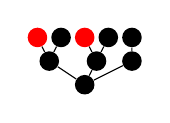
\begin{tikzpicture}[scale=.2]
\node[circle, scale=0.75, fill] (tid0) at (3.75,0){};
\node[circle, scale=0.75, fill] (tid1) at (1.5,1.5){};
\node[circle, scale=0.75, fill, red] (tid4) at (0.75,3){};
\node[circle, scale=0.75, fill] (tid5) at (2.25,3){};
\draw[](tid1) -- (tid4);
\draw[](tid1) -- (tid5);
\node[circle, scale=0.75, fill] (tid2) at (4.5,1.5){};
\node[circle, scale=0.75, fill, red] (tid6) at (3.75,3){};
\node[circle, scale=0.75, fill] (tid7) at (5.25,3){};
\draw[](tid2) -- (tid6);
\draw[](tid2) -- (tid7);
\node[circle, scale=0.75, fill] (tid3) at (6.75,1.5){};
\node[circle, scale=0.75, fill] (tid8) at (6.75,3){};
\draw[](tid3) -- (tid8);
\draw[](tid0) -- (tid1);
\draw[](tid0) -- (tid2);
\draw[](tid0) -- (tid3);

\end{tikzpicture}
\nodepart{two}
\footnotesize{5.625}
};
\node[draw=black, rectangle split, rectangle split parts=2] (sn0x8a8c6c8W-35) at (-35, -36) {
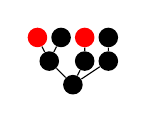
\begin{tikzpicture}[scale=.2]
\node[circle, scale=0.75, fill] (tid0) at (3,0){};
\node[circle, scale=0.75, fill] (tid1) at (1.5,1.5){};
\node[circle, scale=0.75, fill, red] (tid4) at (0.75,3){};
\node[circle, scale=0.75, fill] (tid5) at (2.25,3){};
\draw[](tid1) -- (tid4);
\draw[](tid1) -- (tid5);
\node[circle, scale=0.75, fill] (tid2) at (3.75,1.5){};
\node[circle, scale=0.75, fill, red] (tid6) at (3.75,3){};
\draw[](tid2) -- (tid6);
\node[circle, scale=0.75, fill] (tid3) at (5.25,1.5){};
\node[circle, scale=0.75, fill] (tid7) at (5.25,3){};
\draw[](tid3) -- (tid7);
\draw[](tid0) -- (tid1);
\draw[](tid0) -- (tid2);
\draw[](tid0) -- (tid3);

\end{tikzpicture}
\nodepart{two}
\footnotesize{5.125}
};
\node[draw=black, rectangle split, rectangle split parts=2] (sn0x8a8ffd8W-22) at (-22.5, -48) {
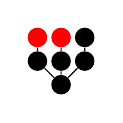
\begin{tikzpicture}[scale=.2]
\node[circle, scale=0.75, fill] (tid0) at (2.25,0){};
\node[circle, scale=0.75, fill] (tid1) at (0.75,1.5){};
\node[circle, scale=0.75, fill, red] (tid4) at (0.75,3){};
\draw[](tid1) -- (tid4);
\node[circle, scale=0.75, fill] (tid2) at (2.25,1.5){};
\node[circle, scale=0.75, fill, red] (tid5) at (2.25,3){};
\draw[](tid2) -- (tid5);
\node[circle, scale=0.75, fill] (tid3) at (3.75,1.5){};
\node[circle, scale=0.75, fill] (tid6) at (3.75,3){};
\draw[](tid3) -- (tid6);
\draw[](tid0) -- (tid1);
\draw[](tid0) -- (tid2);
\draw[](tid0) -- (tid3);

\end{tikzpicture}
\nodepart{two}
\footnotesize{4.625}
};
\node[draw=black, rectangle split, rectangle split parts=2] (sn0x8a90750W-7) at (-7.25, -60) {
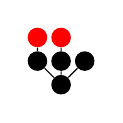
\begin{tikzpicture}[scale=.2]
\node[circle, scale=0.75, fill] (tid0) at (2.25,0){};
\node[circle, scale=0.75, fill] (tid1) at (0.75,1.5){};
\node[circle, scale=0.75, fill, red] (tid4) at (0.75,3){};
\draw[](tid1) -- (tid4);
\node[circle, scale=0.75, fill] (tid2) at (2.25,1.5){};
\node[circle, scale=0.75, fill, red] (tid5) at (2.25,3){};
\draw[](tid2) -- (tid5);
\node[circle, scale=0.75, fill] (tid3) at (3.75,1.5){};
\draw[](tid0) -- (tid1);
\draw[](tid0) -- (tid2);
\draw[](tid0) -- (tid3);

\end{tikzpicture}
\nodepart{two}
\footnotesize{4.125}
};
\node[draw=black, rectangle split, rectangle split parts=2] (sn0x8a90a10W-3) at (-3.25, -72) {
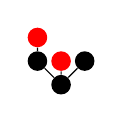
\begin{tikzpicture}[scale=.2]
\node[circle, scale=0.75, fill] (tid0) at (2.25,0){};
\node[circle, scale=0.75, fill] (tid1) at (0.75,1.5){};
\node[circle, scale=0.75, fill, red] (tid4) at (0.75,3){};
\draw[](tid1) -- (tid4);
\node[circle, scale=0.75, fill, red] (tid2) at (2.25,1.5){};
\node[circle, scale=0.75, fill] (tid3) at (3.75,1.5){};
\draw[](tid0) -- (tid1);
\draw[](tid0) -- (tid2);
\draw[](tid0) -- (tid3);

\end{tikzpicture}
\nodepart{two}
\footnotesize{3.625}
};
\node[draw=black, rectangle split, rectangle split parts=2] (sn0x8a90990W-5) at (-5.75, -84) {
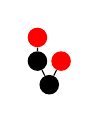
\begin{tikzpicture}[scale=.2]
\node[circle, scale=0.75, fill] (tid0) at (1.5,0){};
\node[circle, scale=0.75, fill] (tid1) at (0.75,1.5){};
\node[circle, scale=0.75, fill, red] (tid3) at (0.75,3){};
\draw[](tid1) -- (tid3);
\node[circle, scale=0.75, fill, red] (tid2) at (2.25,1.5){};
\draw[](tid0) -- (tid1);
\draw[](tid0) -- (tid2);

\end{tikzpicture}
\nodepart{two}
\footnotesize{3.25}
};
\node[draw=black, rectangle split, rectangle split parts=2] (sn0x8a90d40W-4) at (-4.25, -96) {
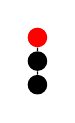
\begin{tikzpicture}[scale=.2]
\node[circle, scale=0.75, fill] (tid0) at (0.75,0){};
\node[circle, scale=0.75, fill] (tid1) at (0.75,1.5){};
\node[circle, scale=0.75, fill, red] (tid2) at (0.75,3){};
\draw[](tid1) -- (tid2);
\draw[](tid0) -- (tid1);

\end{tikzpicture}
\nodepart{two}
\footnotesize{3}
};
\node[draw=black, rectangle split, rectangle split parts=2] (sn0x8a91148W-1) at (-1.75, -108) {

\begin{tikzpicture}[scale=.2]
\node[circle, scale=0.75, fill] (tid0) at (0.75,0){};
\node[circle, scale=0.75, fill, red] (tid1) at (0.75,1.5){};
\draw[](tid0) -- (tid1);

\end{tikzpicture}
\nodepart{two}
\footnotesize{2}
};
\node[draw=black, rectangle split, rectangle split parts=2] (sn0x8a911b0W-1) at (-1.75, -120) {

\begin{tikzpicture}[scale=.2]
\node[circle, scale=0.75, fill, red] (tid0) at (0.75,0){};

\end{tikzpicture}
\nodepart{two}
\footnotesize{1}
};
\draw (sn0x8a91148W-1.south) -- (sn0x8a911b0W-1.north);
\draw (sn0x8a90d40W-4.south) -- (sn0x8a91148W-1.north);
\node[draw=black, rectangle split, rectangle split parts=2] (sn0x8a90ff8W0) at (-0.75, -96) {

\begin{tikzpicture}[scale=.2]
\node[circle, scale=0.75, fill] (tid0) at (1.5,0){};
\node[circle, scale=0.75, fill, red] (tid1) at (0.75,1.5){};
\node[circle, scale=0.75, fill, red] (tid2) at (2.25,1.5){};
\draw[](tid0) -- (tid1);
\draw[](tid0) -- (tid2);

\end{tikzpicture}
\nodepart{two}
\footnotesize{2.5}
};
\draw (sn0x8a90ff8W0.south) -- (sn0x8a91148W-1.north);
\draw (sn0x8a90990W-5.south) -- (sn0x8a90d40W-4.north);
\draw (sn0x8a90990W-5.south) -- (sn0x8a90ff8W0.north);
\node[draw=black, rectangle split, rectangle split parts=2] (sn0x8a90cd8W0) at (-0.75, -84) {
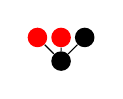
\begin{tikzpicture}[scale=.2]
\node[circle, scale=0.75, fill] (tid0) at (2.25,0){};
\node[circle, scale=0.75, fill, red] (tid1) at (0.75,1.5){};
\node[circle, scale=0.75, fill, red] (tid2) at (2.25,1.5){};
\node[circle, scale=0.75, fill] (tid3) at (3.75,1.5){};
\draw[](tid0) -- (tid1);
\draw[](tid0) -- (tid2);
\draw[](tid0) -- (tid3);

\end{tikzpicture}
\nodepart{two}
\footnotesize{3}
};
\draw (sn0x8a90cd8W0.south) -- (sn0x8a90ff8W0.north);
\draw (sn0x8a90a10W-3.south) -- (sn0x8a90990W-5.north);
\draw (sn0x8a90a10W-3.south) -- (sn0x8a90cd8W0.north);
\draw (sn0x8a90750W-7.south) -- (sn0x8a90a10W-3.north);
\draw (sn0x8a8ffd8W-22.south) -- (sn0x8a90750W-7.north);
\node[draw=black, rectangle split, rectangle split parts=2] (sn0x8a901a0W-16) at (-16, -48) {
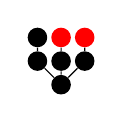
\begin{tikzpicture}[scale=.2]
\node[circle, scale=0.75, fill] (tid0) at (2.25,0){};
\node[circle, scale=0.75, fill] (tid1) at (0.75,1.5){};
\node[circle, scale=0.75, fill] (tid4) at (0.75,3){};
\draw[](tid1) -- (tid4);
\node[circle, scale=0.75, fill] (tid2) at (2.25,1.5){};
\node[circle, scale=0.75, fill, red] (tid5) at (2.25,3){};
\draw[](tid2) -- (tid5);
\node[circle, scale=0.75, fill] (tid3) at (3.75,1.5){};
\node[circle, scale=0.75, fill, red] (tid6) at (3.75,3){};
\draw[](tid3) -- (tid6);
\draw[](tid0) -- (tid1);
\draw[](tid0) -- (tid2);
\draw[](tid0) -- (tid3);

\end{tikzpicture}
\nodepart{two}
\footnotesize{4.625}
};
\draw (sn0x8a901a0W-16.south) -- (sn0x8a90750W-7.north);
\node[draw=black, rectangle split, rectangle split parts=2] (sn0x8a904b8W-9) at (-9.5, -48) {
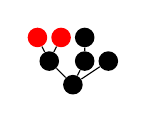
\begin{tikzpicture}[scale=.2]
\node[circle, scale=0.75, fill] (tid0) at (3,0){};
\node[circle, scale=0.75, fill] (tid1) at (1.5,1.5){};
\node[circle, scale=0.75, fill, red] (tid4) at (0.75,3){};
\node[circle, scale=0.75, fill, red] (tid5) at (2.25,3){};
\draw[](tid1) -- (tid4);
\draw[](tid1) -- (tid5);
\node[circle, scale=0.75, fill] (tid2) at (3.75,1.5){};
\node[circle, scale=0.75, fill] (tid6) at (3.75,3){};
\draw[](tid2) -- (tid6);
\node[circle, scale=0.75, fill] (tid3) at (5.25,1.5){};
\draw[](tid0) -- (tid1);
\draw[](tid0) -- (tid2);
\draw[](tid0) -- (tid3);

\end{tikzpicture}
\nodepart{two}
\footnotesize{4.625}
};
\draw (sn0x8a904b8W-9.south) -- (sn0x8a90750W-7.north);
\node[draw=black, rectangle split, rectangle split parts=2] (sn0x8a90520W-1) at (-1.5, -48) {
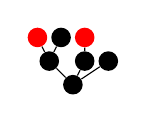
\begin{tikzpicture}[scale=.2]
\node[circle, scale=0.75, fill] (tid0) at (3,0){};
\node[circle, scale=0.75, fill] (tid1) at (1.5,1.5){};
\node[circle, scale=0.75, fill, red] (tid4) at (0.75,3){};
\node[circle, scale=0.75, fill] (tid5) at (2.25,3){};
\draw[](tid1) -- (tid4);
\draw[](tid1) -- (tid5);
\node[circle, scale=0.75, fill] (tid2) at (3.75,1.5){};
\node[circle, scale=0.75, fill, red] (tid6) at (3.75,3){};
\draw[](tid2) -- (tid6);
\node[circle, scale=0.75, fill] (tid3) at (5.25,1.5){};
\draw[](tid0) -- (tid1);
\draw[](tid0) -- (tid2);
\draw[](tid0) -- (tid3);

\end{tikzpicture}
\nodepart{two}
\footnotesize{4.625}
};
\node[draw=black, rectangle split, rectangle split parts=2] (sn0x8a91378W0) at (-0.75, -60) {
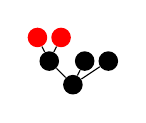
\begin{tikzpicture}[scale=.2]
\node[circle, scale=0.75, fill] (tid0) at (3,0){};
\node[circle, scale=0.75, fill] (tid1) at (1.5,1.5){};
\node[circle, scale=0.75, fill, red] (tid4) at (0.75,3){};
\node[circle, scale=0.75, fill, red] (tid5) at (2.25,3){};
\draw[](tid1) -- (tid4);
\draw[](tid1) -- (tid5);
\node[circle, scale=0.75, fill] (tid2) at (3.75,1.5){};
\node[circle, scale=0.75, fill] (tid3) at (5.25,1.5){};
\draw[](tid0) -- (tid1);
\draw[](tid0) -- (tid2);
\draw[](tid0) -- (tid3);

\end{tikzpicture}
\nodepart{two}
\footnotesize{4.125}
};
\draw (sn0x8a91378W0.south) -- (sn0x8a90a10W-3.north);
\draw (sn0x8a90520W-1.south) -- (sn0x8a90750W-7.north);
\draw (sn0x8a90520W-1.south) -- (sn0x8a91378W0.north);
\draw (sn0x8a8c6c8W-35.south) -- (sn0x8a8ffd8W-22.north);
\draw (sn0x8a8c6c8W-35.south) -- (sn0x8a901a0W-16.north);
\draw (sn0x8a8c6c8W-35.south) -- (sn0x8a904b8W-9.north);
\draw (sn0x8a8c6c8W-35.south) -- (sn0x8a90520W-1.north);
\node[draw=black, rectangle split, rectangle split parts=2] (sn0x8a8b588W-27) at (-27, -36) {
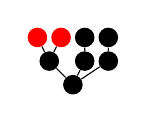
\begin{tikzpicture}[scale=.2]
\node[circle, scale=0.75, fill] (tid0) at (3,0){};
\node[circle, scale=0.75, fill] (tid1) at (1.5,1.5){};
\node[circle, scale=0.75, fill, red] (tid4) at (0.75,3){};
\node[circle, scale=0.75, fill, red] (tid5) at (2.25,3){};
\draw[](tid1) -- (tid4);
\draw[](tid1) -- (tid5);
\node[circle, scale=0.75, fill] (tid2) at (3.75,1.5){};
\node[circle, scale=0.75, fill] (tid6) at (3.75,3){};
\draw[](tid2) -- (tid6);
\node[circle, scale=0.75, fill] (tid3) at (5.25,1.5){};
\node[circle, scale=0.75, fill] (tid7) at (5.25,3){};
\draw[](tid3) -- (tid7);
\draw[](tid0) -- (tid1);
\draw[](tid0) -- (tid2);
\draw[](tid0) -- (tid3);

\end{tikzpicture}
\nodepart{two}
\footnotesize{5.125}
};
\node[draw=black, rectangle split, rectangle split parts=2] (sn0x8a91d08W6) at (6.5, -48) {
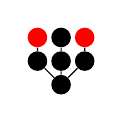
\begin{tikzpicture}[scale=.2]
\node[circle, scale=0.75, fill] (tid0) at (2.25,0){};
\node[circle, scale=0.75, fill] (tid1) at (0.75,1.5){};
\node[circle, scale=0.75, fill, red] (tid4) at (0.75,3){};
\draw[](tid1) -- (tid4);
\node[circle, scale=0.75, fill] (tid2) at (2.25,1.5){};
\node[circle, scale=0.75, fill] (tid5) at (2.25,3){};
\draw[](tid2) -- (tid5);
\node[circle, scale=0.75, fill] (tid3) at (3.75,1.5){};
\node[circle, scale=0.75, fill, red] (tid6) at (3.75,3){};
\draw[](tid3) -- (tid6);
\draw[](tid0) -- (tid1);
\draw[](tid0) -- (tid2);
\draw[](tid0) -- (tid3);

\end{tikzpicture}
\nodepart{two}
\footnotesize{4.625}
};
\draw (sn0x8a91d08W6.south) -- (sn0x8a90750W-7.north);
\draw (sn0x8a8b588W-27.south) -- (sn0x8a8ffd8W-22.north);
\draw (sn0x8a8b588W-27.south) -- (sn0x8a91d08W6.north);
\node[draw=black, rectangle split, rectangle split parts=2] (sn0x8a8c108W-19) at (-19, -36) {
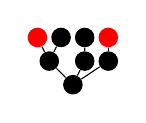
\begin{tikzpicture}[scale=.2]
\node[circle, scale=0.75, fill] (tid0) at (3,0){};
\node[circle, scale=0.75, fill] (tid1) at (1.5,1.5){};
\node[circle, scale=0.75, fill, red] (tid4) at (0.75,3){};
\node[circle, scale=0.75, fill] (tid5) at (2.25,3){};
\draw[](tid1) -- (tid4);
\draw[](tid1) -- (tid5);
\node[circle, scale=0.75, fill] (tid2) at (3.75,1.5){};
\node[circle, scale=0.75, fill] (tid6) at (3.75,3){};
\draw[](tid2) -- (tid6);
\node[circle, scale=0.75, fill] (tid3) at (5.25,1.5){};
\node[circle, scale=0.75, fill, red] (tid7) at (5.25,3){};
\draw[](tid3) -- (tid7);
\draw[](tid0) -- (tid1);
\draw[](tid0) -- (tid2);
\draw[](tid0) -- (tid3);

\end{tikzpicture}
\nodepart{two}
\footnotesize{5.125}
};
\draw (sn0x8a8c108W-19.south) -- (sn0x8a91d08W6.north);
\draw (sn0x8a8c108W-19.south) -- (sn0x8a901a0W-16.north);
\draw (sn0x8a8c108W-19.south) -- (sn0x8a904b8W-9.north);
\draw (sn0x8a8c108W-19.south) -- (sn0x8a90520W-1.north);
\draw (sn0x8a8b730W-28.south) -- (sn0x8a8c6c8W-35.north);
\draw (sn0x8a8b730W-28.south) -- (sn0x8a8b588W-27.north);
\draw (sn0x8a8b730W-28.south) -- (sn0x8a8c108W-19.north);
\draw[draw opacity=0] (sn0x8a8b730W-28.south) -- node[draw opacity=1, anchor=base, draw=black, fill=white]{\footnotesize{0.33}}(sn0x8a8c6c8W-35.north);
\draw[draw opacity=0] (sn0x8a8b730W-28.south) -- node[draw opacity=1, anchor=base, draw=black, fill=white]{\footnotesize{0.33}}(sn0x8a8b588W-27.north);
\draw[draw opacity=0] (sn0x8a8b730W-28.south) -- node[draw opacity=1, anchor=base, draw=black, fill=white]{\footnotesize{0.33}}(sn0x8a8c108W-19.north);
\node[draw=black, rectangle split, rectangle split parts=2] (sn0x8a8a428W-19) at (-19, -24) {
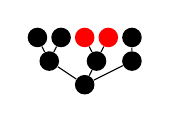
\begin{tikzpicture}[scale=.2]
\node[circle, scale=0.75, fill] (tid0) at (3.75,0){};
\node[circle, scale=0.75, fill] (tid1) at (1.5,1.5){};
\node[circle, scale=0.75, fill] (tid4) at (0.75,3){};
\node[circle, scale=0.75, fill] (tid5) at (2.25,3){};
\draw[](tid1) -- (tid4);
\draw[](tid1) -- (tid5);
\node[circle, scale=0.75, fill] (tid2) at (4.5,1.5){};
\node[circle, scale=0.75, fill, red] (tid6) at (3.75,3){};
\node[circle, scale=0.75, fill, red] (tid7) at (5.25,3){};
\draw[](tid2) -- (tid6);
\draw[](tid2) -- (tid7);
\node[circle, scale=0.75, fill] (tid3) at (6.75,1.5){};
\node[circle, scale=0.75, fill] (tid8) at (6.75,3){};
\draw[](tid3) -- (tid8);
\draw[](tid0) -- (tid1);
\draw[](tid0) -- (tid2);
\draw[](tid0) -- (tid3);

\end{tikzpicture}
\nodepart{two}
\footnotesize{5.6}
};
\node[draw=black, rectangle split, rectangle split parts=2] (sn0x8a91f58W-11) at (-11, -36) {
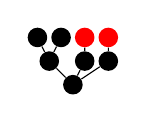
\begin{tikzpicture}[scale=.2]
\node[circle, scale=0.75, fill] (tid0) at (3,0){};
\node[circle, scale=0.75, fill] (tid1) at (1.5,1.5){};
\node[circle, scale=0.75, fill] (tid4) at (0.75,3){};
\node[circle, scale=0.75, fill] (tid5) at (2.25,3){};
\draw[](tid1) -- (tid4);
\draw[](tid1) -- (tid5);
\node[circle, scale=0.75, fill] (tid2) at (3.75,1.5){};
\node[circle, scale=0.75, fill, red] (tid6) at (3.75,3){};
\draw[](tid2) -- (tid6);
\node[circle, scale=0.75, fill] (tid3) at (5.25,1.5){};
\node[circle, scale=0.75, fill, red] (tid7) at (5.25,3){};
\draw[](tid3) -- (tid7);
\draw[](tid0) -- (tid1);
\draw[](tid0) -- (tid2);
\draw[](tid0) -- (tid3);

\end{tikzpicture}
\nodepart{two}
\footnotesize{5.1}
};
\draw (sn0x8a91f58W-11.south) -- (sn0x8a90520W-1.north);
\draw (sn0x8a8a428W-19.south) -- (sn0x8a8c6c8W-35.north);
\draw (sn0x8a8a428W-19.south) -- (sn0x8a91f58W-11.north);
\draw[draw opacity=0] (sn0x8a8a428W-19.south) -- node[draw opacity=1, anchor=base, draw=black, fill=white]{\footnotesize{0.67}}(sn0x8a8c6c8W-35.north);
\draw[draw opacity=0] (sn0x8a8a428W-19.south) -- node[draw opacity=1, anchor=base, draw=black, fill=white]{\footnotesize{0.33}}(sn0x8a91f58W-11.north);
\node[draw=black, rectangle split, rectangle split parts=2] (sn0x8a8ccd8W-9) at (-9.5, -24) {
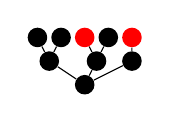
\begin{tikzpicture}[scale=.2]
\node[circle, scale=0.75, fill] (tid0) at (3.75,0){};
\node[circle, scale=0.75, fill] (tid1) at (1.5,1.5){};
\node[circle, scale=0.75, fill] (tid4) at (0.75,3){};
\node[circle, scale=0.75, fill] (tid5) at (2.25,3){};
\draw[](tid1) -- (tid4);
\draw[](tid1) -- (tid5);
\node[circle, scale=0.75, fill] (tid2) at (4.5,1.5){};
\node[circle, scale=0.75, fill, red] (tid6) at (3.75,3){};
\node[circle, scale=0.75, fill] (tid7) at (5.25,3){};
\draw[](tid2) -- (tid6);
\draw[](tid2) -- (tid7);
\node[circle, scale=0.75, fill] (tid3) at (6.75,1.5){};
\node[circle, scale=0.75, fill, red] (tid8) at (6.75,3){};
\draw[](tid3) -- (tid8);
\draw[](tid0) -- (tid1);
\draw[](tid0) -- (tid2);
\draw[](tid0) -- (tid3);

\end{tikzpicture}
\nodepart{two}
\footnotesize{5.6}
};
\node[draw=black, rectangle split, rectangle split parts=2] (sn0x8a921b0W-3) at (-3, -36) {
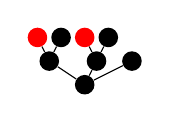
\begin{tikzpicture}[scale=.2]
\node[circle, scale=0.75, fill] (tid0) at (3.75,0){};
\node[circle, scale=0.75, fill] (tid1) at (1.5,1.5){};
\node[circle, scale=0.75, fill, red] (tid4) at (0.75,3){};
\node[circle, scale=0.75, fill] (tid5) at (2.25,3){};
\draw[](tid1) -- (tid4);
\draw[](tid1) -- (tid5);
\node[circle, scale=0.75, fill] (tid2) at (4.5,1.5){};
\node[circle, scale=0.75, fill, red] (tid6) at (3.75,3){};
\node[circle, scale=0.75, fill] (tid7) at (5.25,3){};
\draw[](tid2) -- (tid6);
\draw[](tid2) -- (tid7);
\node[circle, scale=0.75, fill] (tid3) at (6.75,1.5){};
\draw[](tid0) -- (tid1);
\draw[](tid0) -- (tid2);
\draw[](tid0) -- (tid3);

\end{tikzpicture}
\nodepart{two}
\footnotesize{5.1}
};
\draw (sn0x8a921b0W-3.south) -- (sn0x8a90520W-1.north);
\draw (sn0x8a921b0W-3.south) -- (sn0x8a904b8W-9.north);
\node[draw=black, rectangle split, rectangle split parts=2] (sn0x8a924c0W6) at (6.5, -36) {
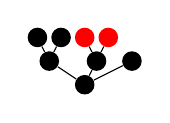
\begin{tikzpicture}[scale=.2]
\node[circle, scale=0.75, fill] (tid0) at (3.75,0){};
\node[circle, scale=0.75, fill] (tid1) at (1.5,1.5){};
\node[circle, scale=0.75, fill] (tid4) at (0.75,3){};
\node[circle, scale=0.75, fill] (tid5) at (2.25,3){};
\draw[](tid1) -- (tid4);
\draw[](tid1) -- (tid5);
\node[circle, scale=0.75, fill] (tid2) at (4.5,1.5){};
\node[circle, scale=0.75, fill, red] (tid6) at (3.75,3){};
\node[circle, scale=0.75, fill, red] (tid7) at (5.25,3){};
\draw[](tid2) -- (tid6);
\draw[](tid2) -- (tid7);
\node[circle, scale=0.75, fill] (tid3) at (6.75,1.5){};
\draw[](tid0) -- (tid1);
\draw[](tid0) -- (tid2);
\draw[](tid0) -- (tid3);

\end{tikzpicture}
\nodepart{two}
\footnotesize{5.1}
};
\draw (sn0x8a924c0W6.south) -- (sn0x8a90520W-1.north);
\draw (sn0x8a8ccd8W-9.south) -- (sn0x8a8c108W-19.north);
\draw (sn0x8a8ccd8W-9.south) -- (sn0x8a91f58W-11.north);
\draw (sn0x8a8ccd8W-9.south) -- (sn0x8a921b0W-3.north);
\draw (sn0x8a8ccd8W-9.south) -- (sn0x8a924c0W6.north);
\draw[draw opacity=0] (sn0x8a8ccd8W-9.south) -- node[draw opacity=1, anchor=base, draw=black, fill=white]{\footnotesize{0.33}}(sn0x8a8c108W-19.north);
\draw[draw opacity=0] (sn0x8a8ccd8W-9.south) -- node[draw opacity=1, anchor=base, draw=black, fill=white]{\footnotesize{0.17}}(sn0x8a91f58W-11.north);
\draw[draw opacity=0] (sn0x8a8ccd8W-9.south) -- node[draw opacity=1, anchor=base, draw=black, fill=white]{\footnotesize{0.33}}(sn0x8a921b0W-3.north);
\draw[draw opacity=0] (sn0x8a8ccd8W-9.south) -- node[draw opacity=1, anchor=base, draw=black, fill=white]{\footnotesize{0.17}}(sn0x8a924c0W6.north);
\node[draw=black, rectangle split, rectangle split parts=2] (sn0x8a8ac98W0) at (0, -24) {
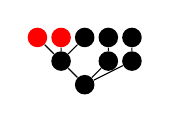
\begin{tikzpicture}[scale=.2]
\node[circle, scale=0.75, fill] (tid0) at (3.75,0){};
\node[circle, scale=0.75, fill] (tid1) at (2.25,1.5){};
\node[circle, scale=0.75, fill, red] (tid4) at (0.75,3){};
\node[circle, scale=0.75, fill, red] (tid5) at (2.25,3){};
\node[circle, scale=0.75, fill] (tid6) at (3.75,3){};
\draw[](tid1) -- (tid4);
\draw[](tid1) -- (tid5);
\draw[](tid1) -- (tid6);
\node[circle, scale=0.75, fill] (tid2) at (5.25,1.5){};
\node[circle, scale=0.75, fill] (tid7) at (5.25,3){};
\draw[](tid2) -- (tid7);
\node[circle, scale=0.75, fill] (tid3) at (6.75,1.5){};
\node[circle, scale=0.75, fill] (tid8) at (6.75,3){};
\draw[](tid3) -- (tid8);
\draw[](tid0) -- (tid1);
\draw[](tid0) -- (tid2);
\draw[](tid0) -- (tid3);

\end{tikzpicture}
\nodepart{two}
\footnotesize{5.6}
};
\draw (sn0x8a8ac98W0.south) -- (sn0x8a8b588W-27.north);
\draw (sn0x8a8ac98W0.south) -- (sn0x8a8c6c8W-35.north);
\draw (sn0x8a8ac98W0.south) -- (sn0x8a8c108W-19.north);
\draw[draw opacity=0] (sn0x8a8ac98W0.south) -- node[draw opacity=1, anchor=base, draw=black, fill=white]{\footnotesize{0.33}}(sn0x8a8b588W-27.north);
\draw[draw opacity=0] (sn0x8a8ac98W0.south) -- node[draw opacity=1, anchor=base, draw=black, fill=white]{\footnotesize{0.33}}(sn0x8a8c6c8W-35.north);
\draw[draw opacity=0] (sn0x8a8ac98W0.south) -- node[draw opacity=1, anchor=base, draw=black, fill=white]{\footnotesize{0.33}}(sn0x8a8c108W-19.north);
\node[draw=black, rectangle split, rectangle split parts=2] (sn0x8a8c7e0W9) at (9.5, -24) {
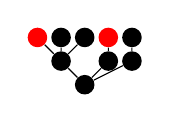
\begin{tikzpicture}[scale=.2]
\node[circle, scale=0.75, fill] (tid0) at (3.75,0){};
\node[circle, scale=0.75, fill] (tid1) at (2.25,1.5){};
\node[circle, scale=0.75, fill, red] (tid4) at (0.75,3){};
\node[circle, scale=0.75, fill] (tid5) at (2.25,3){};
\node[circle, scale=0.75, fill] (tid6) at (3.75,3){};
\draw[](tid1) -- (tid4);
\draw[](tid1) -- (tid5);
\draw[](tid1) -- (tid6);
\node[circle, scale=0.75, fill] (tid2) at (5.25,1.5){};
\node[circle, scale=0.75, fill, red] (tid7) at (5.25,3){};
\draw[](tid2) -- (tid7);
\node[circle, scale=0.75, fill] (tid3) at (6.75,1.5){};
\node[circle, scale=0.75, fill] (tid8) at (6.75,3){};
\draw[](tid3) -- (tid8);
\draw[](tid0) -- (tid1);
\draw[](tid0) -- (tid2);
\draw[](tid0) -- (tid3);

\end{tikzpicture}
\nodepart{two}
\footnotesize{5.6}
};
\node[draw=black, rectangle split, rectangle split parts=2] (sn0x8a928b0W16) at (16, -36) {
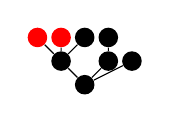
\begin{tikzpicture}[scale=.2]
\node[circle, scale=0.75, fill] (tid0) at (3.75,0){};
\node[circle, scale=0.75, fill] (tid1) at (2.25,1.5){};
\node[circle, scale=0.75, fill, red] (tid4) at (0.75,3){};
\node[circle, scale=0.75, fill, red] (tid5) at (2.25,3){};
\node[circle, scale=0.75, fill] (tid6) at (3.75,3){};
\draw[](tid1) -- (tid4);
\draw[](tid1) -- (tid5);
\draw[](tid1) -- (tid6);
\node[circle, scale=0.75, fill] (tid2) at (5.25,1.5){};
\node[circle, scale=0.75, fill] (tid7) at (5.25,3){};
\draw[](tid2) -- (tid7);
\node[circle, scale=0.75, fill] (tid3) at (6.75,1.5){};
\draw[](tid0) -- (tid1);
\draw[](tid0) -- (tid2);
\draw[](tid0) -- (tid3);

\end{tikzpicture}
\nodepart{two}
\footnotesize{5.1}
};
\draw (sn0x8a928b0W16.south) -- (sn0x8a904b8W-9.north);
\draw (sn0x8a928b0W16.south) -- (sn0x8a90520W-1.north);
\node[draw=black, rectangle split, rectangle split parts=2] (sn0x8a92c50W25) at (26, -36) {
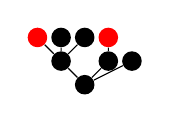
\begin{tikzpicture}[scale=.2]
\node[circle, scale=0.75, fill] (tid0) at (3.75,0){};
\node[circle, scale=0.75, fill] (tid1) at (2.25,1.5){};
\node[circle, scale=0.75, fill, red] (tid4) at (0.75,3){};
\node[circle, scale=0.75, fill] (tid5) at (2.25,3){};
\node[circle, scale=0.75, fill] (tid6) at (3.75,3){};
\draw[](tid1) -- (tid4);
\draw[](tid1) -- (tid5);
\draw[](tid1) -- (tid6);
\node[circle, scale=0.75, fill] (tid2) at (5.25,1.5){};
\node[circle, scale=0.75, fill, red] (tid7) at (5.25,3){};
\draw[](tid2) -- (tid7);
\node[circle, scale=0.75, fill] (tid3) at (6.75,1.5){};
\draw[](tid0) -- (tid1);
\draw[](tid0) -- (tid2);
\draw[](tid0) -- (tid3);

\end{tikzpicture}
\nodepart{two}
\footnotesize{5.1}
};
\node[draw=black, rectangle split, rectangle split parts=2] (sn0x8a92e48W13) at (13, -48) {
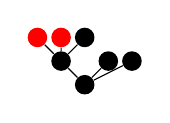
\begin{tikzpicture}[scale=.2]
\node[circle, scale=0.75, fill] (tid0) at (3.75,0){};
\node[circle, scale=0.75, fill] (tid1) at (2.25,1.5){};
\node[circle, scale=0.75, fill, red] (tid4) at (0.75,3){};
\node[circle, scale=0.75, fill, red] (tid5) at (2.25,3){};
\node[circle, scale=0.75, fill] (tid6) at (3.75,3){};
\draw[](tid1) -- (tid4);
\draw[](tid1) -- (tid5);
\draw[](tid1) -- (tid6);
\node[circle, scale=0.75, fill] (tid2) at (5.25,1.5){};
\node[circle, scale=0.75, fill] (tid3) at (6.75,1.5){};
\draw[](tid0) -- (tid1);
\draw[](tid0) -- (tid2);
\draw[](tid0) -- (tid3);

\end{tikzpicture}
\nodepart{two}
\footnotesize{4.6}
};
\draw (sn0x8a92e48W13.south) -- (sn0x8a91378W0.north);
\draw (sn0x8a92c50W25.south) -- (sn0x8a90520W-1.north);
\draw (sn0x8a92c50W25.south) -- (sn0x8a92e48W13.north);
\draw (sn0x8a8c7e0W9.south) -- (sn0x8a8c6c8W-35.north);
\draw (sn0x8a8c7e0W9.south) -- (sn0x8a91f58W-11.north);
\draw (sn0x8a8c7e0W9.south) -- (sn0x8a928b0W16.north);
\draw (sn0x8a8c7e0W9.south) -- (sn0x8a92c50W25.north);
\draw[draw opacity=0] (sn0x8a8c7e0W9.south) -- node[draw opacity=1, anchor=base, draw=black, fill=white]{\footnotesize{0.33}}(sn0x8a8c6c8W-35.north);
\draw[draw opacity=0] (sn0x8a8c7e0W9.south) -- node[draw opacity=1, anchor=base, draw=black, fill=white]{\footnotesize{0.17}}(sn0x8a91f58W-11.north);
\draw[draw opacity=0] (sn0x8a8c7e0W9.south) -- node[draw opacity=1, anchor=base, draw=black, fill=white]{\footnotesize{0.33}}(sn0x8a928b0W16.north);
\draw[draw opacity=0] (sn0x8a8c7e0W9.south) -- node[draw opacity=1, anchor=base, draw=black, fill=white]{\footnotesize{0.17}}(sn0x8a92c50W25.north);
\node[draw=black, rectangle split, rectangle split parts=2] (sn0x8a8caa8W19) at (19, -24) {
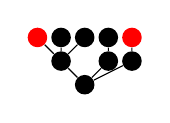
\begin{tikzpicture}[scale=.2]
\node[circle, scale=0.75, fill] (tid0) at (3.75,0){};
\node[circle, scale=0.75, fill] (tid1) at (2.25,1.5){};
\node[circle, scale=0.75, fill, red] (tid4) at (0.75,3){};
\node[circle, scale=0.75, fill] (tid5) at (2.25,3){};
\node[circle, scale=0.75, fill] (tid6) at (3.75,3){};
\draw[](tid1) -- (tid4);
\draw[](tid1) -- (tid5);
\draw[](tid1) -- (tid6);
\node[circle, scale=0.75, fill] (tid2) at (5.25,1.5){};
\node[circle, scale=0.75, fill] (tid7) at (5.25,3){};
\draw[](tid2) -- (tid7);
\node[circle, scale=0.75, fill] (tid3) at (6.75,1.5){};
\node[circle, scale=0.75, fill, red] (tid8) at (6.75,3){};
\draw[](tid3) -- (tid8);
\draw[](tid0) -- (tid1);
\draw[](tid0) -- (tid2);
\draw[](tid0) -- (tid3);

\end{tikzpicture}
\nodepart{two}
\footnotesize{5.6}
};
\draw (sn0x8a8caa8W19.south) -- (sn0x8a8c108W-19.north);
\draw (sn0x8a8caa8W19.south) -- (sn0x8a91f58W-11.north);
\draw (sn0x8a8caa8W19.south) -- (sn0x8a928b0W16.north);
\draw (sn0x8a8caa8W19.south) -- (sn0x8a92c50W25.north);
\draw[draw opacity=0] (sn0x8a8caa8W19.south) -- node[draw opacity=1, anchor=base, draw=black, fill=white]{\footnotesize{0.33}}(sn0x8a8c108W-19.north);
\draw[draw opacity=0] (sn0x8a8caa8W19.south) -- node[draw opacity=1, anchor=base, draw=black, fill=white]{\footnotesize{0.17}}(sn0x8a91f58W-11.north);
\draw[draw opacity=0] (sn0x8a8caa8W19.south) -- node[draw opacity=1, anchor=base, draw=black, fill=white]{\footnotesize{0.33}}(sn0x8a928b0W16.north);
\draw[draw opacity=0] (sn0x8a8caa8W19.south) -- node[draw opacity=1, anchor=base, draw=black, fill=white]{\footnotesize{0.17}}(sn0x8a92c50W25.north);
\draw (sn0x8a8b990W-5.south) -- (sn0x8a8b730W-28.north);
\draw (sn0x8a8b990W-5.south) -- (sn0x8a8a428W-19.north);
\draw (sn0x8a8b990W-5.south) -- (sn0x8a8ccd8W-9.north);
\draw (sn0x8a8b990W-5.south) -- (sn0x8a8ac98W0.north);
\draw (sn0x8a8b990W-5.south) -- (sn0x8a8c7e0W9.north);
\draw (sn0x8a8b990W-5.south) -- (sn0x8a8caa8W19.north);
\draw[draw opacity=0] (sn0x8a8b990W-5.south) -- node[draw opacity=1, anchor=base, draw=black, fill=white]{\footnotesize{0.25}}(sn0x8a8b730W-28.north);
\draw[draw opacity=0] (sn0x8a8b990W-5.south) -- node[draw opacity=1, anchor=base, draw=black, fill=white]{\footnotesize{0.12}}(sn0x8a8a428W-19.north);
\draw[draw opacity=0] (sn0x8a8b990W-5.south) -- node[draw opacity=1, anchor=base, draw=black, fill=white]{\footnotesize{0.12}}(sn0x8a8ccd8W-9.north);
\draw[draw opacity=0] (sn0x8a8b990W-5.south) -- node[draw opacity=1, anchor=base, draw=black, fill=white]{\footnotesize{0.25}}(sn0x8a8ac98W0.north);
\draw[draw opacity=0] (sn0x8a8b990W-5.south) -- node[draw opacity=1, anchor=base, draw=black, fill=white]{\footnotesize{0.12}}(sn0x8a8c7e0W9.north);
\draw[draw opacity=0] (sn0x8a8b990W-5.south) -- node[draw opacity=1, anchor=base, draw=black, fill=white]{\footnotesize{0.12}}(sn0x8a8caa8W19.north);
\end{tikzpicture}

%%% Local Variables:
%%% TeX-master: "thesis/thesis.tex"
%%% End: 

\begin{tikzpicture}[scale=.2, anchor=south west]
\node[draw=black, rectangle split, rectangle split parts=2] (sn0x8a8b9f0W-5) at (-5.5, -12) {
\begin{tikzpicture}[scale=.2]
\node[circle, scale=0.75, fill] (tid0) at (4.5,0){};
\node[circle, scale=0.75, fill] (tid1) at (2.25,1.5){};
\node[circle, scale=0.75, fill, red] (tid4) at (0.75,3){};
\node[circle, scale=0.75, fill, red] (tid5) at (2.25,3){};
\node[circle, scale=0.75, fill] (tid6) at (3.75,3){};
\draw[](tid1) -- (tid4);
\draw[](tid1) -- (tid5);
\draw[](tid1) -- (tid6);
\node[circle, scale=0.75, fill] (tid2) at (6,1.5){};
\node[circle, scale=0.75, fill] (tid7) at (5.25,3){};
\node[circle, scale=0.75, fill] (tid8) at (6.75,3){};
\draw[](tid2) -- (tid7);
\draw[](tid2) -- (tid8);
\node[circle, scale=0.75, fill] (tid3) at (8.25,1.5){};
\node[circle, scale=0.75, fill] (tid9) at (8.25,3){};
\draw[](tid3) -- (tid9);
\draw[](tid0) -- (tid1);
\draw[](tid0) -- (tid2);
\draw[](tid0) -- (tid3);

\end{tikzpicture}
\nodepart{two}
\footnotesize{6.125}
};
\node[draw=black, rectangle split, rectangle split parts=2] (sn0x8a93650W-14) at (-14.25, -24) {
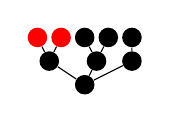
\begin{tikzpicture}[scale=.2]
\node[circle, scale=0.75, fill] (tid0) at (3.75,0){};
\node[circle, scale=0.75, fill] (tid1) at (1.5,1.5){};
\node[circle, scale=0.75, fill, red] (tid4) at (0.75,3){};
\node[circle, scale=0.75, fill, red] (tid5) at (2.25,3){};
\draw[](tid1) -- (tid4);
\draw[](tid1) -- (tid5);
\node[circle, scale=0.75, fill] (tid2) at (4.5,1.5){};
\node[circle, scale=0.75, fill] (tid6) at (3.75,3){};
\node[circle, scale=0.75, fill] (tid7) at (5.25,3){};
\draw[](tid2) -- (tid6);
\draw[](tid2) -- (tid7);
\node[circle, scale=0.75, fill] (tid3) at (6.75,1.5){};
\node[circle, scale=0.75, fill] (tid8) at (6.75,3){};
\draw[](tid3) -- (tid8);
\draw[](tid0) -- (tid1);
\draw[](tid0) -- (tid2);
\draw[](tid0) -- (tid3);

\end{tikzpicture}
\nodepart{two}
\footnotesize{5.625}
};
\node[draw=black, rectangle split, rectangle split parts=2] (sn0x8a8c6c8W-25) at (-25.5, -36) {
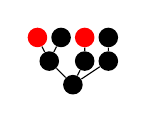
\begin{tikzpicture}[scale=.2]
\node[circle, scale=0.75, fill] (tid0) at (3,0){};
\node[circle, scale=0.75, fill] (tid1) at (1.5,1.5){};
\node[circle, scale=0.75, fill, red] (tid4) at (0.75,3){};
\node[circle, scale=0.75, fill] (tid5) at (2.25,3){};
\draw[](tid1) -- (tid4);
\draw[](tid1) -- (tid5);
\node[circle, scale=0.75, fill] (tid2) at (3.75,1.5){};
\node[circle, scale=0.75, fill, red] (tid6) at (3.75,3){};
\draw[](tid2) -- (tid6);
\node[circle, scale=0.75, fill] (tid3) at (5.25,1.5){};
\node[circle, scale=0.75, fill] (tid7) at (5.25,3){};
\draw[](tid3) -- (tid7);
\draw[](tid0) -- (tid1);
\draw[](tid0) -- (tid2);
\draw[](tid0) -- (tid3);

\end{tikzpicture}
\nodepart{two}
\footnotesize{5.125}
};
\node[draw=black, rectangle split, rectangle split parts=2] (sn0x8a8ffd8W-17) at (-17.75, -48) {
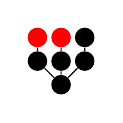
\begin{tikzpicture}[scale=.2]
\node[circle, scale=0.75, fill] (tid0) at (2.25,0){};
\node[circle, scale=0.75, fill] (tid1) at (0.75,1.5){};
\node[circle, scale=0.75, fill, red] (tid4) at (0.75,3){};
\draw[](tid1) -- (tid4);
\node[circle, scale=0.75, fill] (tid2) at (2.25,1.5){};
\node[circle, scale=0.75, fill, red] (tid5) at (2.25,3){};
\draw[](tid2) -- (tid5);
\node[circle, scale=0.75, fill] (tid3) at (3.75,1.5){};
\node[circle, scale=0.75, fill] (tid6) at (3.75,3){};
\draw[](tid3) -- (tid6);
\draw[](tid0) -- (tid1);
\draw[](tid0) -- (tid2);
\draw[](tid0) -- (tid3);

\end{tikzpicture}
\nodepart{two}
\footnotesize{4.625}
};
\node[draw=black, rectangle split, rectangle split parts=2] (sn0x8a90750W-7) at (-7.25, -60) {
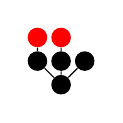
\begin{tikzpicture}[scale=.2]
\node[circle, scale=0.75, fill] (tid0) at (2.25,0){};
\node[circle, scale=0.75, fill] (tid1) at (0.75,1.5){};
\node[circle, scale=0.75, fill, red] (tid4) at (0.75,3){};
\draw[](tid1) -- (tid4);
\node[circle, scale=0.75, fill] (tid2) at (2.25,1.5){};
\node[circle, scale=0.75, fill, red] (tid5) at (2.25,3){};
\draw[](tid2) -- (tid5);
\node[circle, scale=0.75, fill] (tid3) at (3.75,1.5){};
\draw[](tid0) -- (tid1);
\draw[](tid0) -- (tid2);
\draw[](tid0) -- (tid3);

\end{tikzpicture}
\nodepart{two}
\footnotesize{4.125}
};
\node[draw=black, rectangle split, rectangle split parts=2] (sn0x8a90a10W-3) at (-3.25, -72) {
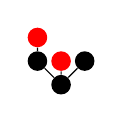
\begin{tikzpicture}[scale=.2]
\node[circle, scale=0.75, fill] (tid0) at (2.25,0){};
\node[circle, scale=0.75, fill] (tid1) at (0.75,1.5){};
\node[circle, scale=0.75, fill, red] (tid4) at (0.75,3){};
\draw[](tid1) -- (tid4);
\node[circle, scale=0.75, fill, red] (tid2) at (2.25,1.5){};
\node[circle, scale=0.75, fill] (tid3) at (3.75,1.5){};
\draw[](tid0) -- (tid1);
\draw[](tid0) -- (tid2);
\draw[](tid0) -- (tid3);

\end{tikzpicture}
\nodepart{two}
\footnotesize{3.625}
};
\node[draw=black, rectangle split, rectangle split parts=2] (sn0x8a90990W-5) at (-5.75, -84) {
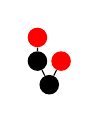
\begin{tikzpicture}[scale=.2]
\node[circle, scale=0.75, fill] (tid0) at (1.5,0){};
\node[circle, scale=0.75, fill] (tid1) at (0.75,1.5){};
\node[circle, scale=0.75, fill, red] (tid3) at (0.75,3){};
\draw[](tid1) -- (tid3);
\node[circle, scale=0.75, fill, red] (tid2) at (2.25,1.5){};
\draw[](tid0) -- (tid1);
\draw[](tid0) -- (tid2);

\end{tikzpicture}
\nodepart{two}
\footnotesize{3.25}
};
\node[draw=black, rectangle split, rectangle split parts=2] (sn0x8a90d40W-4) at (-4.25, -96) {
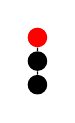
\begin{tikzpicture}[scale=.2]
\node[circle, scale=0.75, fill] (tid0) at (0.75,0){};
\node[circle, scale=0.75, fill] (tid1) at (0.75,1.5){};
\node[circle, scale=0.75, fill, red] (tid2) at (0.75,3){};
\draw[](tid1) -- (tid2);
\draw[](tid0) -- (tid1);

\end{tikzpicture}
\nodepart{two}
\footnotesize{3}
};
\node[draw=black, rectangle split, rectangle split parts=2] (sn0x8a91148W-1) at (-1.75, -108) {

\begin{tikzpicture}[scale=.2]
\node[circle, scale=0.75, fill] (tid0) at (0.75,0){};
\node[circle, scale=0.75, fill, red] (tid1) at (0.75,1.5){};
\draw[](tid0) -- (tid1);

\end{tikzpicture}
\nodepart{two}
\footnotesize{2}
};
\node[draw=black, rectangle split, rectangle split parts=2] (sn0x8a911b0W-1) at (-1.75, -120) {

\begin{tikzpicture}[scale=.2]
\node[circle, scale=0.75, fill, red] (tid0) at (0.75,0){};

\end{tikzpicture}
\nodepart{two}
\footnotesize{1}
};
\draw (sn0x8a91148W-1.south) -- (sn0x8a911b0W-1.north);
\draw (sn0x8a90d40W-4.south) -- (sn0x8a91148W-1.north);
\node[draw=black, rectangle split, rectangle split parts=2] (sn0x8a90ff8W0) at (-0.75, -96) {

\begin{tikzpicture}[scale=.2]
\node[circle, scale=0.75, fill] (tid0) at (1.5,0){};
\node[circle, scale=0.75, fill, red] (tid1) at (0.75,1.5){};
\node[circle, scale=0.75, fill, red] (tid2) at (2.25,1.5){};
\draw[](tid0) -- (tid1);
\draw[](tid0) -- (tid2);

\end{tikzpicture}
\nodepart{two}
\footnotesize{2.5}
};
\draw (sn0x8a90ff8W0.south) -- (sn0x8a91148W-1.north);
\draw (sn0x8a90990W-5.south) -- (sn0x8a90d40W-4.north);
\draw (sn0x8a90990W-5.south) -- (sn0x8a90ff8W0.north);
\node[draw=black, rectangle split, rectangle split parts=2] (sn0x8a90cd8W0) at (-0.75, -84) {
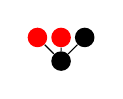
\begin{tikzpicture}[scale=.2]
\node[circle, scale=0.75, fill] (tid0) at (2.25,0){};
\node[circle, scale=0.75, fill, red] (tid1) at (0.75,1.5){};
\node[circle, scale=0.75, fill, red] (tid2) at (2.25,1.5){};
\node[circle, scale=0.75, fill] (tid3) at (3.75,1.5){};
\draw[](tid0) -- (tid1);
\draw[](tid0) -- (tid2);
\draw[](tid0) -- (tid3);

\end{tikzpicture}
\nodepart{two}
\footnotesize{3}
};
\draw (sn0x8a90cd8W0.south) -- (sn0x8a90ff8W0.north);
\draw (sn0x8a90a10W-3.south) -- (sn0x8a90990W-5.north);
\draw (sn0x8a90a10W-3.south) -- (sn0x8a90cd8W0.north);
\draw (sn0x8a90750W-7.south) -- (sn0x8a90a10W-3.north);
\draw (sn0x8a8ffd8W-17.south) -- (sn0x8a90750W-7.north);
\node[draw=black, rectangle split, rectangle split parts=2] (sn0x8a901a0W-11) at (-11.25, -48) {
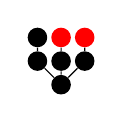
\begin{tikzpicture}[scale=.2]
\node[circle, scale=0.75, fill] (tid0) at (2.25,0){};
\node[circle, scale=0.75, fill] (tid1) at (0.75,1.5){};
\node[circle, scale=0.75, fill] (tid4) at (0.75,3){};
\draw[](tid1) -- (tid4);
\node[circle, scale=0.75, fill] (tid2) at (2.25,1.5){};
\node[circle, scale=0.75, fill, red] (tid5) at (2.25,3){};
\draw[](tid2) -- (tid5);
\node[circle, scale=0.75, fill] (tid3) at (3.75,1.5){};
\node[circle, scale=0.75, fill, red] (tid6) at (3.75,3){};
\draw[](tid3) -- (tid6);
\draw[](tid0) -- (tid1);
\draw[](tid0) -- (tid2);
\draw[](tid0) -- (tid3);

\end{tikzpicture}
\nodepart{two}
\footnotesize{4.625}
};
\draw (sn0x8a901a0W-11.south) -- (sn0x8a90750W-7.north);
\node[draw=black, rectangle split, rectangle split parts=2] (sn0x8a904b8W-4) at (-4.75, -48) {
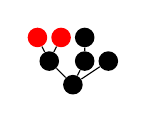
\begin{tikzpicture}[scale=.2]
\node[circle, scale=0.75, fill] (tid0) at (3,0){};
\node[circle, scale=0.75, fill] (tid1) at (1.5,1.5){};
\node[circle, scale=0.75, fill, red] (tid4) at (0.75,3){};
\node[circle, scale=0.75, fill, red] (tid5) at (2.25,3){};
\draw[](tid1) -- (tid4);
\draw[](tid1) -- (tid5);
\node[circle, scale=0.75, fill] (tid2) at (3.75,1.5){};
\node[circle, scale=0.75, fill] (tid6) at (3.75,3){};
\draw[](tid2) -- (tid6);
\node[circle, scale=0.75, fill] (tid3) at (5.25,1.5){};
\draw[](tid0) -- (tid1);
\draw[](tid0) -- (tid2);
\draw[](tid0) -- (tid3);

\end{tikzpicture}
\nodepart{two}
\footnotesize{4.625}
};
\draw (sn0x8a904b8W-4.south) -- (sn0x8a90750W-7.north);
\node[draw=black, rectangle split, rectangle split parts=2] (sn0x8a90520W3) at (3.25, -48) {
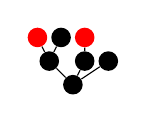
\begin{tikzpicture}[scale=.2]
\node[circle, scale=0.75, fill] (tid0) at (3,0){};
\node[circle, scale=0.75, fill] (tid1) at (1.5,1.5){};
\node[circle, scale=0.75, fill, red] (tid4) at (0.75,3){};
\node[circle, scale=0.75, fill] (tid5) at (2.25,3){};
\draw[](tid1) -- (tid4);
\draw[](tid1) -- (tid5);
\node[circle, scale=0.75, fill] (tid2) at (3.75,1.5){};
\node[circle, scale=0.75, fill, red] (tid6) at (3.75,3){};
\draw[](tid2) -- (tid6);
\node[circle, scale=0.75, fill] (tid3) at (5.25,1.5){};
\draw[](tid0) -- (tid1);
\draw[](tid0) -- (tid2);
\draw[](tid0) -- (tid3);

\end{tikzpicture}
\nodepart{two}
\footnotesize{4.625}
};
\node[draw=black, rectangle split, rectangle split parts=2] (sn0x8a91378W0) at (-0.75, -60) {
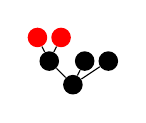
\begin{tikzpicture}[scale=.2]
\node[circle, scale=0.75, fill] (tid0) at (3,0){};
\node[circle, scale=0.75, fill] (tid1) at (1.5,1.5){};
\node[circle, scale=0.75, fill, red] (tid4) at (0.75,3){};
\node[circle, scale=0.75, fill, red] (tid5) at (2.25,3){};
\draw[](tid1) -- (tid4);
\draw[](tid1) -- (tid5);
\node[circle, scale=0.75, fill] (tid2) at (3.75,1.5){};
\node[circle, scale=0.75, fill] (tid3) at (5.25,1.5){};
\draw[](tid0) -- (tid1);
\draw[](tid0) -- (tid2);
\draw[](tid0) -- (tid3);

\end{tikzpicture}
\nodepart{two}
\footnotesize{4.125}
};
\draw (sn0x8a91378W0.south) -- (sn0x8a90a10W-3.north);
\draw (sn0x8a90520W3.south) -- (sn0x8a90750W-7.north);
\draw (sn0x8a90520W3.south) -- (sn0x8a91378W0.north);
\draw (sn0x8a8c6c8W-25.south) -- (sn0x8a8ffd8W-17.north);
\draw (sn0x8a8c6c8W-25.south) -- (sn0x8a901a0W-11.north);
\draw (sn0x8a8c6c8W-25.south) -- (sn0x8a904b8W-4.north);
\draw (sn0x8a8c6c8W-25.south) -- (sn0x8a90520W3.north);
\node[draw=black, rectangle split, rectangle split parts=2] (sn0x8a91f58W-17) at (-17.5, -36) {
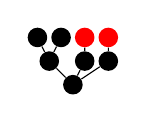
\begin{tikzpicture}[scale=.2]
\node[circle, scale=0.75, fill] (tid0) at (3,0){};
\node[circle, scale=0.75, fill] (tid1) at (1.5,1.5){};
\node[circle, scale=0.75, fill] (tid4) at (0.75,3){};
\node[circle, scale=0.75, fill] (tid5) at (2.25,3){};
\draw[](tid1) -- (tid4);
\draw[](tid1) -- (tid5);
\node[circle, scale=0.75, fill] (tid2) at (3.75,1.5){};
\node[circle, scale=0.75, fill, red] (tid6) at (3.75,3){};
\draw[](tid2) -- (tid6);
\node[circle, scale=0.75, fill] (tid3) at (5.25,1.5){};
\node[circle, scale=0.75, fill, red] (tid7) at (5.25,3){};
\draw[](tid3) -- (tid7);
\draw[](tid0) -- (tid1);
\draw[](tid0) -- (tid2);
\draw[](tid0) -- (tid3);

\end{tikzpicture}
\nodepart{two}
\footnotesize{5.125}
};
\draw (sn0x8a91f58W-17.south) -- (sn0x8a90520W3.north);
\draw (sn0x8a93650W-14.south) -- (sn0x8a8c6c8W-25.north);
\draw (sn0x8a93650W-14.south) -- (sn0x8a91f58W-17.north);
\draw[draw opacity=0] (sn0x8a93650W-14.south) -- node[draw opacity=1, anchor=base, draw=black, fill=white]{\footnotesize{0.67}}(sn0x8a8c6c8W-25.north);
\draw[draw opacity=0] (sn0x8a93650W-14.south) -- node[draw opacity=1, anchor=base, draw=black, fill=white]{\footnotesize{0.33}}(sn0x8a91f58W-17.north);
\node[draw=black, rectangle split, rectangle split parts=2] (sn0x8a8b730W-4) at (-4.8, -24) {
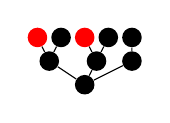
\begin{tikzpicture}[scale=.2]
\node[circle, scale=0.75, fill] (tid0) at (3.75,0){};
\node[circle, scale=0.75, fill] (tid1) at (1.5,1.5){};
\node[circle, scale=0.75, fill, red] (tid4) at (0.75,3){};
\node[circle, scale=0.75, fill] (tid5) at (2.25,3){};
\draw[](tid1) -- (tid4);
\draw[](tid1) -- (tid5);
\node[circle, scale=0.75, fill] (tid2) at (4.5,1.5){};
\node[circle, scale=0.75, fill, red] (tid6) at (3.75,3){};
\node[circle, scale=0.75, fill] (tid7) at (5.25,3){};
\draw[](tid2) -- (tid6);
\draw[](tid2) -- (tid7);
\node[circle, scale=0.75, fill] (tid3) at (6.75,1.5){};
\node[circle, scale=0.75, fill] (tid8) at (6.75,3){};
\draw[](tid3) -- (tid8);
\draw[](tid0) -- (tid1);
\draw[](tid0) -- (tid2);
\draw[](tid0) -- (tid3);

\end{tikzpicture}
\nodepart{two}
\footnotesize{5.6}
};
\node[draw=black, rectangle split, rectangle split parts=2] (sn0x8a8b588W-9) at (-9.5, -36) {
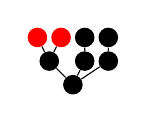
\begin{tikzpicture}[scale=.2]
\node[circle, scale=0.75, fill] (tid0) at (3,0){};
\node[circle, scale=0.75, fill] (tid1) at (1.5,1.5){};
\node[circle, scale=0.75, fill, red] (tid4) at (0.75,3){};
\node[circle, scale=0.75, fill, red] (tid5) at (2.25,3){};
\draw[](tid1) -- (tid4);
\draw[](tid1) -- (tid5);
\node[circle, scale=0.75, fill] (tid2) at (3.75,1.5){};
\node[circle, scale=0.75, fill] (tid6) at (3.75,3){};
\draw[](tid2) -- (tid6);
\node[circle, scale=0.75, fill] (tid3) at (5.25,1.5){};
\node[circle, scale=0.75, fill] (tid7) at (5.25,3){};
\draw[](tid3) -- (tid7);
\draw[](tid0) -- (tid1);
\draw[](tid0) -- (tid2);
\draw[](tid0) -- (tid3);

\end{tikzpicture}
\nodepart{two}
\footnotesize{5.1}
};
\node[draw=black, rectangle split, rectangle split parts=2] (sn0x8a91d08W11) at (11, -48) {
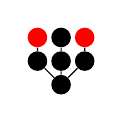
\begin{tikzpicture}[scale=.2]
\node[circle, scale=0.75, fill] (tid0) at (2.25,0){};
\node[circle, scale=0.75, fill] (tid1) at (0.75,1.5){};
\node[circle, scale=0.75, fill, red] (tid4) at (0.75,3){};
\draw[](tid1) -- (tid4);
\node[circle, scale=0.75, fill] (tid2) at (2.25,1.5){};
\node[circle, scale=0.75, fill] (tid5) at (2.25,3){};
\draw[](tid2) -- (tid5);
\node[circle, scale=0.75, fill] (tid3) at (3.75,1.5){};
\node[circle, scale=0.75, fill, red] (tid6) at (3.75,3){};
\draw[](tid3) -- (tid6);
\draw[](tid0) -- (tid1);
\draw[](tid0) -- (tid2);
\draw[](tid0) -- (tid3);

\end{tikzpicture}
\nodepart{two}
\footnotesize{4.6}
};
\draw (sn0x8a91d08W11.south) -- (sn0x8a90750W-7.north);
\draw (sn0x8a8b588W-9.south) -- (sn0x8a8ffd8W-17.north);
\draw (sn0x8a8b588W-9.south) -- (sn0x8a91d08W11.north);
\node[draw=black, rectangle split, rectangle split parts=2] (sn0x8a8c108W-1) at (-1.5, -36) {
\begin{tikzpicture}[scale=.2]
\node[circle, scale=0.75, fill] (tid0) at (3,0){};
\node[circle, scale=0.75, fill] (tid1) at (1.5,1.5){};
\node[circle, scale=0.75, fill, red] (tid4) at (0.75,3){};
\node[circle, scale=0.75, fill] (tid5) at (2.25,3){};
\draw[](tid1) -- (tid4);
\draw[](tid1) -- (tid5);
\node[circle, scale=0.75, fill] (tid2) at (3.75,1.5){};
\node[circle, scale=0.75, fill] (tid6) at (3.75,3){};
\draw[](tid2) -- (tid6);
\node[circle, scale=0.75, fill] (tid3) at (5.25,1.5){};
\node[circle, scale=0.75, fill, red] (tid7) at (5.25,3){};
\draw[](tid3) -- (tid7);
\draw[](tid0) -- (tid1);
\draw[](tid0) -- (tid2);
\draw[](tid0) -- (tid3);

\end{tikzpicture}
\nodepart{two}
\footnotesize{5.1}
};
\draw (sn0x8a8c108W-1.south) -- (sn0x8a91d08W11.north);
\draw (sn0x8a8c108W-1.south) -- (sn0x8a901a0W-11.north);
\draw (sn0x8a8c108W-1.south) -- (sn0x8a904b8W-4.north);
\draw (sn0x8a8c108W-1.south) -- (sn0x8a90520W3.north);
\draw (sn0x8a8b730W-4.south) -- (sn0x8a8c6c8W-25.north);
\draw (sn0x8a8b730W-4.south) -- (sn0x8a8b588W-9.north);
\draw (sn0x8a8b730W-4.south) -- (sn0x8a8c108W-1.north);
\draw[draw opacity=0] (sn0x8a8b730W-4.south) -- node[draw opacity=1, anchor=base, draw=black, fill=white]{\footnotesize{0.33}}(sn0x8a8c6c8W-25.north);
\draw[draw opacity=0] (sn0x8a8b730W-4.south) -- node[draw opacity=1, anchor=base, draw=black, fill=white]{\footnotesize{0.33}}(sn0x8a8b588W-9.north);
\draw[draw opacity=0] (sn0x8a8b730W-4.south) -- node[draw opacity=1, anchor=base, draw=black, fill=white]{\footnotesize{0.33}}(sn0x8a8c108W-1.north);
\node[draw=black, rectangle split, rectangle split parts=2] (sn0x8a937b0W4) at (4.8, -24) {
\begin{tikzpicture}[scale=.2]
\node[circle, scale=0.75, fill] (tid0) at (3.75,0){};
\node[circle, scale=0.75, fill] (tid1) at (1.5,1.5){};
\node[circle, scale=0.75, fill, red] (tid4) at (0.75,3){};
\node[circle, scale=0.75, fill] (tid5) at (2.25,3){};
\draw[](tid1) -- (tid4);
\draw[](tid1) -- (tid5);
\node[circle, scale=0.75, fill] (tid2) at (4.5,1.5){};
\node[circle, scale=0.75, fill] (tid6) at (3.75,3){};
\node[circle, scale=0.75, fill] (tid7) at (5.25,3){};
\draw[](tid2) -- (tid6);
\draw[](tid2) -- (tid7);
\node[circle, scale=0.75, fill] (tid3) at (6.75,1.5){};
\node[circle, scale=0.75, fill, red] (tid8) at (6.75,3){};
\draw[](tid3) -- (tid8);
\draw[](tid0) -- (tid1);
\draw[](tid0) -- (tid2);
\draw[](tid0) -- (tid3);

\end{tikzpicture}
\nodepart{two}
\footnotesize{5.6}
};
\node[draw=black, rectangle split, rectangle split parts=2] (sn0x8a93b78W6) at (6.5, -36) {
\begin{tikzpicture}[scale=.2]
\node[circle, scale=0.75, fill] (tid0) at (3.75,0){};
\node[circle, scale=0.75, fill] (tid1) at (1.5,1.5){};
\node[circle, scale=0.75, fill, red] (tid4) at (0.75,3){};
\node[circle, scale=0.75, fill, red] (tid5) at (2.25,3){};
\draw[](tid1) -- (tid4);
\draw[](tid1) -- (tid5);
\node[circle, scale=0.75, fill] (tid2) at (4.5,1.5){};
\node[circle, scale=0.75, fill] (tid6) at (3.75,3){};
\node[circle, scale=0.75, fill] (tid7) at (5.25,3){};
\draw[](tid2) -- (tid6);
\draw[](tid2) -- (tid7);
\node[circle, scale=0.75, fill] (tid3) at (6.75,1.5){};
\draw[](tid0) -- (tid1);
\draw[](tid0) -- (tid2);
\draw[](tid0) -- (tid3);

\end{tikzpicture}
\nodepart{two}
\footnotesize{5.1}
};
\draw (sn0x8a93b78W6.south) -- (sn0x8a90520W3.north);
\node[draw=black, rectangle split, rectangle split parts=2] (sn0x8a921b0W16) at (16, -36) {
\begin{tikzpicture}[scale=.2]
\node[circle, scale=0.75, fill] (tid0) at (3.75,0){};
\node[circle, scale=0.75, fill] (tid1) at (1.5,1.5){};
\node[circle, scale=0.75, fill, red] (tid4) at (0.75,3){};
\node[circle, scale=0.75, fill] (tid5) at (2.25,3){};
\draw[](tid1) -- (tid4);
\draw[](tid1) -- (tid5);
\node[circle, scale=0.75, fill] (tid2) at (4.5,1.5){};
\node[circle, scale=0.75, fill, red] (tid6) at (3.75,3){};
\node[circle, scale=0.75, fill] (tid7) at (5.25,3){};
\draw[](tid2) -- (tid6);
\draw[](tid2) -- (tid7);
\node[circle, scale=0.75, fill] (tid3) at (6.75,1.5){};
\draw[](tid0) -- (tid1);
\draw[](tid0) -- (tid2);
\draw[](tid0) -- (tid3);

\end{tikzpicture}
\nodepart{two}
\footnotesize{5.1}
};
\draw (sn0x8a921b0W16.south) -- (sn0x8a90520W3.north);
\draw (sn0x8a921b0W16.south) -- (sn0x8a904b8W-4.north);
\draw (sn0x8a937b0W4.south) -- (sn0x8a91f58W-17.north);
\draw (sn0x8a937b0W4.south) -- (sn0x8a8c108W-1.north);
\draw (sn0x8a937b0W4.south) -- (sn0x8a93b78W6.north);
\draw (sn0x8a937b0W4.south) -- (sn0x8a921b0W16.north);
\draw[draw opacity=0] (sn0x8a937b0W4.south) -- node[draw opacity=1, anchor=base, draw=black, fill=white]{\footnotesize{0.17}}(sn0x8a91f58W-17.north);
\draw[draw opacity=0] (sn0x8a937b0W4.south) -- node[draw opacity=1, anchor=base, draw=black, fill=white]{\footnotesize{0.33}}(sn0x8a8c108W-1.north);
\draw[draw opacity=0] (sn0x8a937b0W4.south) -- node[draw opacity=1, anchor=base, draw=black, fill=white]{\footnotesize{0.17}}(sn0x8a93b78W6.north);
\draw[draw opacity=0] (sn0x8a937b0W4.south) -- node[draw opacity=1, anchor=base, draw=black, fill=white]{\footnotesize{0.33}}(sn0x8a921b0W16.north);
\draw (sn0x8a8b9f0W-5.south) -- (sn0x8a93650W-14.north);
\draw (sn0x8a8b9f0W-5.south) -- (sn0x8a8b730W-4.north);
\draw (sn0x8a8b9f0W-5.south) -- (sn0x8a937b0W4.north);
\draw[draw opacity=0] (sn0x8a8b9f0W-5.south) -- node[draw opacity=1, anchor=base, draw=black, fill=white]{\footnotesize{0.25}}(sn0x8a93650W-14.north);
\draw[draw opacity=0] (sn0x8a8b9f0W-5.south) -- node[draw opacity=1, anchor=base, draw=black, fill=white]{\footnotesize{0.5}}(sn0x8a8b730W-4.north);
\draw[draw opacity=0] (sn0x8a8b9f0W-5.south) -- node[draw opacity=1, anchor=base, draw=black, fill=white]{\footnotesize{0.25}}(sn0x8a937b0W4.north);
\end{tikzpicture}

%%% Local Variables:
%%% TeX-master: "thesis/thesis.tex"
%%% End: 

\begin{tikzpicture}[scale=.2, anchor=south west]
\node[draw=black, rectangle split, rectangle split parts=2] (sn0x8a8ba50W-5) at (-5.5, -12) {
\begin{tikzpicture}[scale=.2]
\node[circle, scale=0.75, fill] (tid0) at (4.5,0){};
\node[circle, scale=0.75, fill] (tid1) at (2.25,1.5){};
\node[circle, scale=0.75, fill, red] (tid4) at (0.75,3){};
\node[circle, scale=0.75, fill] (tid5) at (2.25,3){};
\node[circle, scale=0.75, fill] (tid6) at (3.75,3){};
\draw[](tid1) -- (tid4);
\draw[](tid1) -- (tid5);
\draw[](tid1) -- (tid6);
\node[circle, scale=0.75, fill] (tid2) at (6,1.5){};
\node[circle, scale=0.75, fill] (tid7) at (5.25,3){};
\node[circle, scale=0.75, fill] (tid8) at (6.75,3){};
\draw[](tid2) -- (tid7);
\draw[](tid2) -- (tid8);
\node[circle, scale=0.75, fill] (tid3) at (8.25,1.5){};
\node[circle, scale=0.75, fill, red] (tid9) at (8.25,3){};
\draw[](tid3) -- (tid9);
\draw[](tid0) -- (tid1);
\draw[](tid0) -- (tid2);
\draw[](tid0) -- (tid3);

\end{tikzpicture}
\nodepart{two}
\footnotesize{6.125}
};
\node[draw=black, rectangle split, rectangle split parts=2] (sn0x8a937b0W-20) at (-20.5, -24) {
\begin{tikzpicture}[scale=.2]
\node[circle, scale=0.75, fill] (tid0) at (3.75,0){};
\node[circle, scale=0.75, fill] (tid1) at (1.5,1.5){};
\node[circle, scale=0.75, fill, red] (tid4) at (0.75,3){};
\node[circle, scale=0.75, fill] (tid5) at (2.25,3){};
\draw[](tid1) -- (tid4);
\draw[](tid1) -- (tid5);
\node[circle, scale=0.75, fill] (tid2) at (4.5,1.5){};
\node[circle, scale=0.75, fill] (tid6) at (3.75,3){};
\node[circle, scale=0.75, fill] (tid7) at (5.25,3){};
\draw[](tid2) -- (tid6);
\draw[](tid2) -- (tid7);
\node[circle, scale=0.75, fill] (tid3) at (6.75,1.5){};
\node[circle, scale=0.75, fill, red] (tid8) at (6.75,3){};
\draw[](tid3) -- (tid8);
\draw[](tid0) -- (tid1);
\draw[](tid0) -- (tid2);
\draw[](tid0) -- (tid3);

\end{tikzpicture}
\nodepart{two}
\footnotesize{5.625}
};
\node[draw=black, rectangle split, rectangle split parts=2] (sn0x8a91f58W-31) at (-31.75, -36) {
\begin{tikzpicture}[scale=.2]
\node[circle, scale=0.75, fill] (tid0) at (3,0){};
\node[circle, scale=0.75, fill] (tid1) at (1.5,1.5){};
\node[circle, scale=0.75, fill] (tid4) at (0.75,3){};
\node[circle, scale=0.75, fill] (tid5) at (2.25,3){};
\draw[](tid1) -- (tid4);
\draw[](tid1) -- (tid5);
\node[circle, scale=0.75, fill] (tid2) at (3.75,1.5){};
\node[circle, scale=0.75, fill, red] (tid6) at (3.75,3){};
\draw[](tid2) -- (tid6);
\node[circle, scale=0.75, fill] (tid3) at (5.25,1.5){};
\node[circle, scale=0.75, fill, red] (tid7) at (5.25,3){};
\draw[](tid3) -- (tid7);
\draw[](tid0) -- (tid1);
\draw[](tid0) -- (tid2);
\draw[](tid0) -- (tid3);

\end{tikzpicture}
\nodepart{two}
\footnotesize{5.125}
};
\node[draw=black, rectangle split, rectangle split parts=2] (sn0x8a90520W-19) at (-19.25, -48) {
\begin{tikzpicture}[scale=.2]
\node[circle, scale=0.75, fill] (tid0) at (3,0){};
\node[circle, scale=0.75, fill] (tid1) at (1.5,1.5){};
\node[circle, scale=0.75, fill, red] (tid4) at (0.75,3){};
\node[circle, scale=0.75, fill] (tid5) at (2.25,3){};
\draw[](tid1) -- (tid4);
\draw[](tid1) -- (tid5);
\node[circle, scale=0.75, fill] (tid2) at (3.75,1.5){};
\node[circle, scale=0.75, fill, red] (tid6) at (3.75,3){};
\draw[](tid2) -- (tid6);
\node[circle, scale=0.75, fill] (tid3) at (5.25,1.5){};
\draw[](tid0) -- (tid1);
\draw[](tid0) -- (tid2);
\draw[](tid0) -- (tid3);

\end{tikzpicture}
\nodepart{two}
\footnotesize{4.625}
};
\node[draw=black, rectangle split, rectangle split parts=2] (sn0x8a90750W-7) at (-7.25, -60) {
\begin{tikzpicture}[scale=.2]
\node[circle, scale=0.75, fill] (tid0) at (2.25,0){};
\node[circle, scale=0.75, fill] (tid1) at (0.75,1.5){};
\node[circle, scale=0.75, fill, red] (tid4) at (0.75,3){};
\draw[](tid1) -- (tid4);
\node[circle, scale=0.75, fill] (tid2) at (2.25,1.5){};
\node[circle, scale=0.75, fill, red] (tid5) at (2.25,3){};
\draw[](tid2) -- (tid5);
\node[circle, scale=0.75, fill] (tid3) at (3.75,1.5){};
\draw[](tid0) -- (tid1);
\draw[](tid0) -- (tid2);
\draw[](tid0) -- (tid3);

\end{tikzpicture}
\nodepart{two}
\footnotesize{4.125}
};
\node[draw=black, rectangle split, rectangle split parts=2] (sn0x8a90a10W-3) at (-3.25, -72) {
\begin{tikzpicture}[scale=.2]
\node[circle, scale=0.75, fill] (tid0) at (2.25,0){};
\node[circle, scale=0.75, fill] (tid1) at (0.75,1.5){};
\node[circle, scale=0.75, fill, red] (tid4) at (0.75,3){};
\draw[](tid1) -- (tid4);
\node[circle, scale=0.75, fill, red] (tid2) at (2.25,1.5){};
\node[circle, scale=0.75, fill] (tid3) at (3.75,1.5){};
\draw[](tid0) -- (tid1);
\draw[](tid0) -- (tid2);
\draw[](tid0) -- (tid3);

\end{tikzpicture}
\nodepart{two}
\footnotesize{3.625}
};
\node[draw=black, rectangle split, rectangle split parts=2] (sn0x8a90990W-5) at (-5.75, -84) {
\begin{tikzpicture}[scale=.2]
\node[circle, scale=0.75, fill] (tid0) at (1.5,0){};
\node[circle, scale=0.75, fill] (tid1) at (0.75,1.5){};
\node[circle, scale=0.75, fill, red] (tid3) at (0.75,3){};
\draw[](tid1) -- (tid3);
\node[circle, scale=0.75, fill, red] (tid2) at (2.25,1.5){};
\draw[](tid0) -- (tid1);
\draw[](tid0) -- (tid2);

\end{tikzpicture}
\nodepart{two}
\footnotesize{3.25}
};
\node[draw=black, rectangle split, rectangle split parts=2] (sn0x8a90d40W-4) at (-4.25, -96) {
\begin{tikzpicture}[scale=.2]
\node[circle, scale=0.75, fill] (tid0) at (0.75,0){};
\node[circle, scale=0.75, fill] (tid1) at (0.75,1.5){};
\node[circle, scale=0.75, fill, red] (tid2) at (0.75,3){};
\draw[](tid1) -- (tid2);
\draw[](tid0) -- (tid1);

\end{tikzpicture}
\nodepart{two}
\footnotesize{3}
};
\node[draw=black, rectangle split, rectangle split parts=2] (sn0x8a91148W-1) at (-1.75, -108) {
\begin{tikzpicture}[scale=.2]
\node[circle, scale=0.75, fill] (tid0) at (0.75,0){};
\node[circle, scale=0.75, fill, red] (tid1) at (0.75,1.5){};
\draw[](tid0) -- (tid1);

\end{tikzpicture}
\nodepart{two}
\footnotesize{2}
};
\node[draw=black, rectangle split, rectangle split parts=2] (sn0x8a911b0W-1) at (-1.75, -120) {
\begin{tikzpicture}[scale=.2]
\node[circle, scale=0.75, fill, red] (tid0) at (0.75,0){};

\end{tikzpicture}
\nodepart{two}
\footnotesize{1}
};
\draw (sn0x8a91148W-1.south) -- (sn0x8a911b0W-1.north);
\draw (sn0x8a90d40W-4.south) -- (sn0x8a91148W-1.north);
\node[draw=black, rectangle split, rectangle split parts=2] (sn0x8a90ff8W0) at (-0.75, -96) {
\begin{tikzpicture}[scale=.2]
\node[circle, scale=0.75, fill] (tid0) at (1.5,0){};
\node[circle, scale=0.75, fill, red] (tid1) at (0.75,1.5){};
\node[circle, scale=0.75, fill, red] (tid2) at (2.25,1.5){};
\draw[](tid0) -- (tid1);
\draw[](tid0) -- (tid2);

\end{tikzpicture}
\nodepart{two}
\footnotesize{2.5}
};
\draw (sn0x8a90ff8W0.south) -- (sn0x8a91148W-1.north);
\draw (sn0x8a90990W-5.south) -- (sn0x8a90d40W-4.north);
\draw (sn0x8a90990W-5.south) -- (sn0x8a90ff8W0.north);
\node[draw=black, rectangle split, rectangle split parts=2] (sn0x8a90cd8W0) at (-0.75, -84) {
\begin{tikzpicture}[scale=.2]
\node[circle, scale=0.75, fill] (tid0) at (2.25,0){};
\node[circle, scale=0.75, fill, red] (tid1) at (0.75,1.5){};
\node[circle, scale=0.75, fill, red] (tid2) at (2.25,1.5){};
\node[circle, scale=0.75, fill] (tid3) at (3.75,1.5){};
\draw[](tid0) -- (tid1);
\draw[](tid0) -- (tid2);
\draw[](tid0) -- (tid3);

\end{tikzpicture}
\nodepart{two}
\footnotesize{3}
};
\draw (sn0x8a90cd8W0.south) -- (sn0x8a90ff8W0.north);
\draw (sn0x8a90a10W-3.south) -- (sn0x8a90990W-5.north);
\draw (sn0x8a90a10W-3.south) -- (sn0x8a90cd8W0.north);
\draw (sn0x8a90750W-7.south) -- (sn0x8a90a10W-3.north);
\node[draw=black, rectangle split, rectangle split parts=2] (sn0x8a91378W0) at (-0.75, -60) {
\begin{tikzpicture}[scale=.2]
\node[circle, scale=0.75, fill] (tid0) at (3,0){};
\node[circle, scale=0.75, fill] (tid1) at (1.5,1.5){};
\node[circle, scale=0.75, fill, red] (tid4) at (0.75,3){};
\node[circle, scale=0.75, fill, red] (tid5) at (2.25,3){};
\draw[](tid1) -- (tid4);
\draw[](tid1) -- (tid5);
\node[circle, scale=0.75, fill] (tid2) at (3.75,1.5){};
\node[circle, scale=0.75, fill] (tid3) at (5.25,1.5){};
\draw[](tid0) -- (tid1);
\draw[](tid0) -- (tid2);
\draw[](tid0) -- (tid3);

\end{tikzpicture}
\nodepart{two}
\footnotesize{4.125}
};
\draw (sn0x8a91378W0.south) -- (sn0x8a90a10W-3.north);
\draw (sn0x8a90520W-19.south) -- (sn0x8a90750W-7.north);
\draw (sn0x8a90520W-19.south) -- (sn0x8a91378W0.north);
\draw (sn0x8a91f58W-31.south) -- (sn0x8a90520W-19.north);
\node[draw=black, rectangle split, rectangle split parts=2] (sn0x8a8c108W-23) at (-23.75, -36) {
\begin{tikzpicture}[scale=.2]
\node[circle, scale=0.75, fill] (tid0) at (3,0){};
\node[circle, scale=0.75, fill] (tid1) at (1.5,1.5){};
\node[circle, scale=0.75, fill, red] (tid4) at (0.75,3){};
\node[circle, scale=0.75, fill] (tid5) at (2.25,3){};
\draw[](tid1) -- (tid4);
\draw[](tid1) -- (tid5);
\node[circle, scale=0.75, fill] (tid2) at (3.75,1.5){};
\node[circle, scale=0.75, fill] (tid6) at (3.75,3){};
\draw[](tid2) -- (tid6);
\node[circle, scale=0.75, fill] (tid3) at (5.25,1.5){};
\node[circle, scale=0.75, fill, red] (tid7) at (5.25,3){};
\draw[](tid3) -- (tid7);
\draw[](tid0) -- (tid1);
\draw[](tid0) -- (tid2);
\draw[](tid0) -- (tid3);

\end{tikzpicture}
\nodepart{two}
\footnotesize{5.125}
};
\node[draw=black, rectangle split, rectangle split parts=2] (sn0x8a91d08W-11) at (-11.25, -48) {
\begin{tikzpicture}[scale=.2]
\node[circle, scale=0.75, fill] (tid0) at (2.25,0){};
\node[circle, scale=0.75, fill] (tid1) at (0.75,1.5){};
\node[circle, scale=0.75, fill, red] (tid4) at (0.75,3){};
\draw[](tid1) -- (tid4);
\node[circle, scale=0.75, fill] (tid2) at (2.25,1.5){};
\node[circle, scale=0.75, fill] (tid5) at (2.25,3){};
\draw[](tid2) -- (tid5);
\node[circle, scale=0.75, fill] (tid3) at (3.75,1.5){};
\node[circle, scale=0.75, fill, red] (tid6) at (3.75,3){};
\draw[](tid3) -- (tid6);
\draw[](tid0) -- (tid1);
\draw[](tid0) -- (tid2);
\draw[](tid0) -- (tid3);

\end{tikzpicture}
\nodepart{two}
\footnotesize{4.625}
};
\draw (sn0x8a91d08W-11.south) -- (sn0x8a90750W-7.north);
\node[draw=black, rectangle split, rectangle split parts=2] (sn0x8a901a0W-4) at (-4.75, -48) {
\begin{tikzpicture}[scale=.2]
\node[circle, scale=0.75, fill] (tid0) at (2.25,0){};
\node[circle, scale=0.75, fill] (tid1) at (0.75,1.5){};
\node[circle, scale=0.75, fill] (tid4) at (0.75,3){};
\draw[](tid1) -- (tid4);
\node[circle, scale=0.75, fill] (tid2) at (2.25,1.5){};
\node[circle, scale=0.75, fill, red] (tid5) at (2.25,3){};
\draw[](tid2) -- (tid5);
\node[circle, scale=0.75, fill] (tid3) at (3.75,1.5){};
\node[circle, scale=0.75, fill, red] (tid6) at (3.75,3){};
\draw[](tid3) -- (tid6);
\draw[](tid0) -- (tid1);
\draw[](tid0) -- (tid2);
\draw[](tid0) -- (tid3);

\end{tikzpicture}
\nodepart{two}
\footnotesize{4.625}
};
\draw (sn0x8a901a0W-4.south) -- (sn0x8a90750W-7.north);
\node[draw=black, rectangle split, rectangle split parts=2] (sn0x8a904b8W1) at (1.75, -48) {
\begin{tikzpicture}[scale=.2]
\node[circle, scale=0.75, fill] (tid0) at (3,0){};
\node[circle, scale=0.75, fill] (tid1) at (1.5,1.5){};
\node[circle, scale=0.75, fill, red] (tid4) at (0.75,3){};
\node[circle, scale=0.75, fill, red] (tid5) at (2.25,3){};
\draw[](tid1) -- (tid4);
\draw[](tid1) -- (tid5);
\node[circle, scale=0.75, fill] (tid2) at (3.75,1.5){};
\node[circle, scale=0.75, fill] (tid6) at (3.75,3){};
\draw[](tid2) -- (tid6);
\node[circle, scale=0.75, fill] (tid3) at (5.25,1.5){};
\draw[](tid0) -- (tid1);
\draw[](tid0) -- (tid2);
\draw[](tid0) -- (tid3);

\end{tikzpicture}
\nodepart{two}
\footnotesize{4.625}
};
\draw (sn0x8a904b8W1.south) -- (sn0x8a90750W-7.north);
\draw (sn0x8a8c108W-23.south) -- (sn0x8a91d08W-11.north);
\draw (sn0x8a8c108W-23.south) -- (sn0x8a901a0W-4.north);
\draw (sn0x8a8c108W-23.south) -- (sn0x8a904b8W1.north);
\draw (sn0x8a8c108W-23.south) -- (sn0x8a90520W-19.north);
\node[draw=black, rectangle split, rectangle split parts=2] (sn0x8a93b78W-15) at (-15.75, -36) {
\begin{tikzpicture}[scale=.2]
\node[circle, scale=0.75, fill] (tid0) at (3.75,0){};
\node[circle, scale=0.75, fill] (tid1) at (1.5,1.5){};
\node[circle, scale=0.75, fill, red] (tid4) at (0.75,3){};
\node[circle, scale=0.75, fill, red] (tid5) at (2.25,3){};
\draw[](tid1) -- (tid4);
\draw[](tid1) -- (tid5);
\node[circle, scale=0.75, fill] (tid2) at (4.5,1.5){};
\node[circle, scale=0.75, fill] (tid6) at (3.75,3){};
\node[circle, scale=0.75, fill] (tid7) at (5.25,3){};
\draw[](tid2) -- (tid6);
\draw[](tid2) -- (tid7);
\node[circle, scale=0.75, fill] (tid3) at (6.75,1.5){};
\draw[](tid0) -- (tid1);
\draw[](tid0) -- (tid2);
\draw[](tid0) -- (tid3);

\end{tikzpicture}
\nodepart{two}
\footnotesize{5.125}
};
\draw (sn0x8a93b78W-15.south) -- (sn0x8a90520W-19.north);
\node[draw=black, rectangle split, rectangle split parts=2] (sn0x8a921b0W-6) at (-6.25, -36) {
\begin{tikzpicture}[scale=.2]
\node[circle, scale=0.75, fill] (tid0) at (3.75,0){};
\node[circle, scale=0.75, fill] (tid1) at (1.5,1.5){};
\node[circle, scale=0.75, fill, red] (tid4) at (0.75,3){};
\node[circle, scale=0.75, fill] (tid5) at (2.25,3){};
\draw[](tid1) -- (tid4);
\draw[](tid1) -- (tid5);
\node[circle, scale=0.75, fill] (tid2) at (4.5,1.5){};
\node[circle, scale=0.75, fill, red] (tid6) at (3.75,3){};
\node[circle, scale=0.75, fill] (tid7) at (5.25,3){};
\draw[](tid2) -- (tid6);
\draw[](tid2) -- (tid7);
\node[circle, scale=0.75, fill] (tid3) at (6.75,1.5){};
\draw[](tid0) -- (tid1);
\draw[](tid0) -- (tid2);
\draw[](tid0) -- (tid3);

\end{tikzpicture}
\nodepart{two}
\footnotesize{5.125}
};
\draw (sn0x8a921b0W-6.south) -- (sn0x8a90520W-19.north);
\draw (sn0x8a921b0W-6.south) -- (sn0x8a904b8W1.north);
\draw (sn0x8a937b0W-20.south) -- (sn0x8a91f58W-31.north);
\draw (sn0x8a937b0W-20.south) -- (sn0x8a8c108W-23.north);
\draw (sn0x8a937b0W-20.south) -- (sn0x8a93b78W-15.north);
\draw (sn0x8a937b0W-20.south) -- (sn0x8a921b0W-6.north);
\draw[draw opacity=0] (sn0x8a937b0W-20.south) -- node[draw opacity=1, anchor=base, draw=black, fill=white]{\footnotesize{0.17}}(sn0x8a91f58W-31.north);
\draw[draw opacity=0] (sn0x8a937b0W-20.south) -- node[draw opacity=1, anchor=base, draw=black, fill=white]{\footnotesize{0.33}}(sn0x8a8c108W-23.north);
\draw[draw opacity=0] (sn0x8a937b0W-20.south) -- node[draw opacity=1, anchor=base, draw=black, fill=white]{\footnotesize{0.17}}(sn0x8a93b78W-15.north);
\draw[draw opacity=0] (sn0x8a937b0W-20.south) -- node[draw opacity=1, anchor=base, draw=black, fill=white]{\footnotesize{0.33}}(sn0x8a921b0W-6.north);
\node[draw=black, rectangle split, rectangle split parts=2] (sn0x8a8ccd8W-11) at (-11, -24) {
\begin{tikzpicture}[scale=.2]
\node[circle, scale=0.75, fill] (tid0) at (3.75,0){};
\node[circle, scale=0.75, fill] (tid1) at (1.5,1.5){};
\node[circle, scale=0.75, fill] (tid4) at (0.75,3){};
\node[circle, scale=0.75, fill] (tid5) at (2.25,3){};
\draw[](tid1) -- (tid4);
\draw[](tid1) -- (tid5);
\node[circle, scale=0.75, fill] (tid2) at (4.5,1.5){};
\node[circle, scale=0.75, fill, red] (tid6) at (3.75,3){};
\node[circle, scale=0.75, fill] (tid7) at (5.25,3){};
\draw[](tid2) -- (tid6);
\draw[](tid2) -- (tid7);
\node[circle, scale=0.75, fill] (tid3) at (6.75,1.5){};
\node[circle, scale=0.75, fill, red] (tid8) at (6.75,3){};
\draw[](tid3) -- (tid8);
\draw[](tid0) -- (tid1);
\draw[](tid0) -- (tid2);
\draw[](tid0) -- (tid3);

\end{tikzpicture}
\nodepart{two}
\footnotesize{5.6}
};
\node[draw=black, rectangle split, rectangle split parts=2] (sn0x8a924c0W3) at (3.2, -36) {
\begin{tikzpicture}[scale=.2]
\node[circle, scale=0.75, fill] (tid0) at (3.75,0){};
\node[circle, scale=0.75, fill] (tid1) at (1.5,1.5){};
\node[circle, scale=0.75, fill] (tid4) at (0.75,3){};
\node[circle, scale=0.75, fill] (tid5) at (2.25,3){};
\draw[](tid1) -- (tid4);
\draw[](tid1) -- (tid5);
\node[circle, scale=0.75, fill] (tid2) at (4.5,1.5){};
\node[circle, scale=0.75, fill, red] (tid6) at (3.75,3){};
\node[circle, scale=0.75, fill, red] (tid7) at (5.25,3){};
\draw[](tid2) -- (tid6);
\draw[](tid2) -- (tid7);
\node[circle, scale=0.75, fill] (tid3) at (6.75,1.5){};
\draw[](tid0) -- (tid1);
\draw[](tid0) -- (tid2);
\draw[](tid0) -- (tid3);

\end{tikzpicture}
\nodepart{two}
\footnotesize{5.1}
};
\draw (sn0x8a924c0W3.south) -- (sn0x8a90520W-19.north);
\draw (sn0x8a8ccd8W-11.south) -- (sn0x8a8c108W-23.north);
\draw (sn0x8a8ccd8W-11.south) -- (sn0x8a91f58W-31.north);
\draw (sn0x8a8ccd8W-11.south) -- (sn0x8a921b0W-6.north);
\draw (sn0x8a8ccd8W-11.south) -- (sn0x8a924c0W3.north);
\draw[draw opacity=0] (sn0x8a8ccd8W-11.south) -- node[draw opacity=1, anchor=base, draw=black, fill=white]{\footnotesize{0.33}}(sn0x8a8c108W-23.north);
\draw[draw opacity=0] (sn0x8a8ccd8W-11.south) -- node[draw opacity=1, anchor=base, draw=black, fill=white]{\footnotesize{0.17}}(sn0x8a91f58W-31.north);
\draw[draw opacity=0] (sn0x8a8ccd8W-11.south) -- node[draw opacity=1, anchor=base, draw=black, fill=white]{\footnotesize{0.33}}(sn0x8a921b0W-6.north);
\draw[draw opacity=0] (sn0x8a8ccd8W-11.south) -- node[draw opacity=1, anchor=base, draw=black, fill=white]{\footnotesize{0.17}}(sn0x8a924c0W3.north);
\node[draw=black, rectangle split, rectangle split parts=2] (sn0x8a93df0W-1) at (-1.5, -24) {
\begin{tikzpicture}[scale=.2]
\node[circle, scale=0.75, fill] (tid0) at (4.5,0){};
\node[circle, scale=0.75, fill] (tid1) at (2.25,1.5){};
\node[circle, scale=0.75, fill, red] (tid4) at (0.75,3){};
\node[circle, scale=0.75, fill, red] (tid5) at (2.25,3){};
\node[circle, scale=0.75, fill] (tid6) at (3.75,3){};
\draw[](tid1) -- (tid4);
\draw[](tid1) -- (tid5);
\draw[](tid1) -- (tid6);
\node[circle, scale=0.75, fill] (tid2) at (6,1.5){};
\node[circle, scale=0.75, fill] (tid7) at (5.25,3){};
\node[circle, scale=0.75, fill] (tid8) at (6.75,3){};
\draw[](tid2) -- (tid7);
\draw[](tid2) -- (tid8);
\node[circle, scale=0.75, fill] (tid3) at (8.25,1.5){};
\draw[](tid0) -- (tid1);
\draw[](tid0) -- (tid2);
\draw[](tid0) -- (tid3);

\end{tikzpicture}
\nodepart{two}
\footnotesize{5.6}
};
\draw (sn0x8a93df0W-1.south) -- (sn0x8a93b78W-15.north);
\draw (sn0x8a93df0W-1.south) -- (sn0x8a921b0W-6.north);
\draw[draw opacity=0] (sn0x8a93df0W-1.south) -- node[draw opacity=1, anchor=base, draw=black, fill=white]{\footnotesize{0.33}}(sn0x8a93b78W-15.north);
\draw[draw opacity=0] (sn0x8a93df0W-1.south) -- node[draw opacity=1, anchor=base, draw=black, fill=white]{\footnotesize{0.67}}(sn0x8a921b0W-6.north);
\node[draw=black, rectangle split, rectangle split parts=2] (sn0x8a94218W9) at (9.5, -24) {
\begin{tikzpicture}[scale=.2]
\node[circle, scale=0.75, fill] (tid0) at (4.5,0){};
\node[circle, scale=0.75, fill] (tid1) at (2.25,1.5){};
\node[circle, scale=0.75, fill, red] (tid4) at (0.75,3){};
\node[circle, scale=0.75, fill] (tid5) at (2.25,3){};
\node[circle, scale=0.75, fill] (tid6) at (3.75,3){};
\draw[](tid1) -- (tid4);
\draw[](tid1) -- (tid5);
\draw[](tid1) -- (tid6);
\node[circle, scale=0.75, fill] (tid2) at (6,1.5){};
\node[circle, scale=0.75, fill, red] (tid7) at (5.25,3){};
\node[circle, scale=0.75, fill] (tid8) at (6.75,3){};
\draw[](tid2) -- (tid7);
\draw[](tid2) -- (tid8);
\node[circle, scale=0.75, fill] (tid3) at (8.25,1.5){};
\draw[](tid0) -- (tid1);
\draw[](tid0) -- (tid2);
\draw[](tid0) -- (tid3);

\end{tikzpicture}
\nodepart{two}
\footnotesize{5.6}
};
\node[draw=black, rectangle split, rectangle split parts=2] (sn0x8a928b0W12) at (13, -36) {
\begin{tikzpicture}[scale=.2]
\node[circle, scale=0.75, fill] (tid0) at (3.75,0){};
\node[circle, scale=0.75, fill] (tid1) at (2.25,1.5){};
\node[circle, scale=0.75, fill, red] (tid4) at (0.75,3){};
\node[circle, scale=0.75, fill, red] (tid5) at (2.25,3){};
\node[circle, scale=0.75, fill] (tid6) at (3.75,3){};
\draw[](tid1) -- (tid4);
\draw[](tid1) -- (tid5);
\draw[](tid1) -- (tid6);
\node[circle, scale=0.75, fill] (tid2) at (5.25,1.5){};
\node[circle, scale=0.75, fill] (tid7) at (5.25,3){};
\draw[](tid2) -- (tid7);
\node[circle, scale=0.75, fill] (tid3) at (6.75,1.5){};
\draw[](tid0) -- (tid1);
\draw[](tid0) -- (tid2);
\draw[](tid0) -- (tid3);

\end{tikzpicture}
\nodepart{two}
\footnotesize{5.1}
};
\draw (sn0x8a928b0W12.south) -- (sn0x8a904b8W1.north);
\draw (sn0x8a928b0W12.south) -- (sn0x8a90520W-19.north);
\node[draw=black, rectangle split, rectangle split parts=2] (sn0x8a92c50W22) at (22, -36) {
\begin{tikzpicture}[scale=.2]
\node[circle, scale=0.75, fill] (tid0) at (3.75,0){};
\node[circle, scale=0.75, fill] (tid1) at (2.25,1.5){};
\node[circle, scale=0.75, fill, red] (tid4) at (0.75,3){};
\node[circle, scale=0.75, fill] (tid5) at (2.25,3){};
\node[circle, scale=0.75, fill] (tid6) at (3.75,3){};
\draw[](tid1) -- (tid4);
\draw[](tid1) -- (tid5);
\draw[](tid1) -- (tid6);
\node[circle, scale=0.75, fill] (tid2) at (5.25,1.5){};
\node[circle, scale=0.75, fill, red] (tid7) at (5.25,3){};
\draw[](tid2) -- (tid7);
\node[circle, scale=0.75, fill] (tid3) at (6.75,1.5){};
\draw[](tid0) -- (tid1);
\draw[](tid0) -- (tid2);
\draw[](tid0) -- (tid3);

\end{tikzpicture}
\nodepart{two}
\footnotesize{5.1}
};
\node[draw=black, rectangle split, rectangle split parts=2] (sn0x8a92e48W9) at (9.8, -48) {
\begin{tikzpicture}[scale=.2]
\node[circle, scale=0.75, fill] (tid0) at (3.75,0){};
\node[circle, scale=0.75, fill] (tid1) at (2.25,1.5){};
\node[circle, scale=0.75, fill, red] (tid4) at (0.75,3){};
\node[circle, scale=0.75, fill, red] (tid5) at (2.25,3){};
\node[circle, scale=0.75, fill] (tid6) at (3.75,3){};
\draw[](tid1) -- (tid4);
\draw[](tid1) -- (tid5);
\draw[](tid1) -- (tid6);
\node[circle, scale=0.75, fill] (tid2) at (5.25,1.5){};
\node[circle, scale=0.75, fill] (tid3) at (6.75,1.5){};
\draw[](tid0) -- (tid1);
\draw[](tid0) -- (tid2);
\draw[](tid0) -- (tid3);

\end{tikzpicture}
\nodepart{two}
\footnotesize{4.6}
};
\draw (sn0x8a92e48W9.south) -- (sn0x8a91378W0.north);
\draw (sn0x8a92c50W22.south) -- (sn0x8a90520W-19.north);
\draw (sn0x8a92c50W22.south) -- (sn0x8a92e48W9.north);
\draw (sn0x8a94218W9.south) -- (sn0x8a921b0W-6.north);
\draw (sn0x8a94218W9.south) -- (sn0x8a924c0W3.north);
\draw (sn0x8a94218W9.south) -- (sn0x8a928b0W12.north);
\draw (sn0x8a94218W9.south) -- (sn0x8a92c50W22.north);
\draw[draw opacity=0] (sn0x8a94218W9.south) -- node[draw opacity=1, anchor=base, draw=black, fill=white]{\footnotesize{0.33}}(sn0x8a921b0W-6.north);
\draw[draw opacity=0] (sn0x8a94218W9.south) -- node[draw opacity=1, anchor=base, draw=black, fill=white]{\footnotesize{0.17}}(sn0x8a924c0W3.north);
\draw[draw opacity=0] (sn0x8a94218W9.south) -- node[draw opacity=1, anchor=base, draw=black, fill=white]{\footnotesize{0.33}}(sn0x8a928b0W12.north);
\draw[draw opacity=0] (sn0x8a94218W9.south) -- node[draw opacity=1, anchor=base, draw=black, fill=white]{\footnotesize{0.17}}(sn0x8a92c50W22.north);
\draw (sn0x8a8ba50W-5.south) -- (sn0x8a937b0W-20.north);
\draw (sn0x8a8ba50W-5.south) -- (sn0x8a8ccd8W-11.north);
\draw (sn0x8a8ba50W-5.south) -- (sn0x8a93df0W-1.north);
\draw (sn0x8a8ba50W-5.south) -- (sn0x8a94218W9.north);
\end{tikzpicture}

%%% Local Variables:
%%% TeX-master: "thesis/thesis.tex"
%%% End: 

\begin{tikzpicture}[scale=.2, anchor=south west]
\node[draw=black, rectangle split, rectangle split parts=2] (sn0x8a8bab0W-5) at (-5.5, -12) {
\begin{tikzpicture}[scale=.2]
\node[circle, scale=0.75, fill] (tid0) at (4.5,0){};
\node[circle, scale=0.75, fill] (tid1) at (2.25,1.5){};
\node[circle, scale=0.75, fill] (tid4) at (0.75,3){};
\node[circle, scale=0.75, fill] (tid5) at (2.25,3){};
\node[circle, scale=0.75, fill] (tid6) at (3.75,3){};
\draw[](tid1) -- (tid4);
\draw[](tid1) -- (tid5);
\draw[](tid1) -- (tid6);
\node[circle, scale=0.75, fill] (tid2) at (6,1.5){};
\node[circle, scale=0.75, fill, red] (tid7) at (5.25,3){};
\node[circle, scale=0.75, fill, red] (tid8) at (6.75,3){};
\draw[](tid2) -- (tid7);
\draw[](tid2) -- (tid8);
\node[circle, scale=0.75, fill] (tid3) at (8.25,1.5){};
\node[circle, scale=0.75, fill] (tid9) at (8.25,3){};
\draw[](tid3) -- (tid9);
\draw[](tid0) -- (tid1);
\draw[](tid0) -- (tid2);
\draw[](tid0) -- (tid3);

\end{tikzpicture}
\nodepart{two}
\footnotesize{6.125}
};
\node[draw=black, rectangle split, rectangle split parts=2] (sn0x8a8c7e0W-9) at (-9.5, -24) {
\begin{tikzpicture}[scale=.2]
\node[circle, scale=0.75, fill] (tid0) at (3.75,0){};
\node[circle, scale=0.75, fill] (tid1) at (2.25,1.5){};
\node[circle, scale=0.75, fill, red] (tid4) at (0.75,3){};
\node[circle, scale=0.75, fill] (tid5) at (2.25,3){};
\node[circle, scale=0.75, fill] (tid6) at (3.75,3){};
\draw[](tid1) -- (tid4);
\draw[](tid1) -- (tid5);
\draw[](tid1) -- (tid6);
\node[circle, scale=0.75, fill] (tid2) at (5.25,1.5){};
\node[circle, scale=0.75, fill, red] (tid7) at (5.25,3){};
\draw[](tid2) -- (tid7);
\node[circle, scale=0.75, fill] (tid3) at (6.75,1.5){};
\node[circle, scale=0.75, fill] (tid8) at (6.75,3){};
\draw[](tid3) -- (tid8);
\draw[](tid0) -- (tid1);
\draw[](tid0) -- (tid2);
\draw[](tid0) -- (tid3);

\end{tikzpicture}
\nodepart{two}
\footnotesize{5.625}
};
\node[draw=black, rectangle split, rectangle split parts=2] (sn0x8a8c6c8W-17) at (-17.5, -36) {
\begin{tikzpicture}[scale=.2]
\node[circle, scale=0.75, fill] (tid0) at (3,0){};
\node[circle, scale=0.75, fill] (tid1) at (1.5,1.5){};
\node[circle, scale=0.75, fill, red] (tid4) at (0.75,3){};
\node[circle, scale=0.75, fill] (tid5) at (2.25,3){};
\draw[](tid1) -- (tid4);
\draw[](tid1) -- (tid5);
\node[circle, scale=0.75, fill] (tid2) at (3.75,1.5){};
\node[circle, scale=0.75, fill, red] (tid6) at (3.75,3){};
\draw[](tid2) -- (tid6);
\node[circle, scale=0.75, fill] (tid3) at (5.25,1.5){};
\node[circle, scale=0.75, fill] (tid7) at (5.25,3){};
\draw[](tid3) -- (tid7);
\draw[](tid0) -- (tid1);
\draw[](tid0) -- (tid2);
\draw[](tid0) -- (tid3);

\end{tikzpicture}
\nodepart{two}
\footnotesize{5.125}
};
\node[draw=black, rectangle split, rectangle split parts=2] (sn0x8a8ffd8W-19) at (-19.25, -48) {
\begin{tikzpicture}[scale=.2]
\node[circle, scale=0.75, fill] (tid0) at (2.25,0){};
\node[circle, scale=0.75, fill] (tid1) at (0.75,1.5){};
\node[circle, scale=0.75, fill, red] (tid4) at (0.75,3){};
\draw[](tid1) -- (tid4);
\node[circle, scale=0.75, fill] (tid2) at (2.25,1.5){};
\node[circle, scale=0.75, fill, red] (tid5) at (2.25,3){};
\draw[](tid2) -- (tid5);
\node[circle, scale=0.75, fill] (tid3) at (3.75,1.5){};
\node[circle, scale=0.75, fill] (tid6) at (3.75,3){};
\draw[](tid3) -- (tid6);
\draw[](tid0) -- (tid1);
\draw[](tid0) -- (tid2);
\draw[](tid0) -- (tid3);

\end{tikzpicture}
\nodepart{two}
\footnotesize{4.625}
};
\node[draw=black, rectangle split, rectangle split parts=2] (sn0x8a90750W-7) at (-7.25, -60) {
\begin{tikzpicture}[scale=.2]
\node[circle, scale=0.75, fill] (tid0) at (2.25,0){};
\node[circle, scale=0.75, fill] (tid1) at (0.75,1.5){};
\node[circle, scale=0.75, fill, red] (tid4) at (0.75,3){};
\draw[](tid1) -- (tid4);
\node[circle, scale=0.75, fill] (tid2) at (2.25,1.5){};
\node[circle, scale=0.75, fill, red] (tid5) at (2.25,3){};
\draw[](tid2) -- (tid5);
\node[circle, scale=0.75, fill] (tid3) at (3.75,1.5){};
\draw[](tid0) -- (tid1);
\draw[](tid0) -- (tid2);
\draw[](tid0) -- (tid3);

\end{tikzpicture}
\nodepart{two}
\footnotesize{4.125}
};
\node[draw=black, rectangle split, rectangle split parts=2] (sn0x8a90a10W-3) at (-3.25, -72) {
\begin{tikzpicture}[scale=.2]
\node[circle, scale=0.75, fill] (tid0) at (2.25,0){};
\node[circle, scale=0.75, fill] (tid1) at (0.75,1.5){};
\node[circle, scale=0.75, fill, red] (tid4) at (0.75,3){};
\draw[](tid1) -- (tid4);
\node[circle, scale=0.75, fill, red] (tid2) at (2.25,1.5){};
\node[circle, scale=0.75, fill] (tid3) at (3.75,1.5){};
\draw[](tid0) -- (tid1);
\draw[](tid0) -- (tid2);
\draw[](tid0) -- (tid3);

\end{tikzpicture}
\nodepart{two}
\footnotesize{3.625}
};
\node[draw=black, rectangle split, rectangle split parts=2] (sn0x8a90990W-5) at (-5.75, -84) {
\begin{tikzpicture}[scale=.2]
\node[circle, scale=0.75, fill] (tid0) at (1.5,0){};
\node[circle, scale=0.75, fill] (tid1) at (0.75,1.5){};
\node[circle, scale=0.75, fill, red] (tid3) at (0.75,3){};
\draw[](tid1) -- (tid3);
\node[circle, scale=0.75, fill, red] (tid2) at (2.25,1.5){};
\draw[](tid0) -- (tid1);
\draw[](tid0) -- (tid2);

\end{tikzpicture}
\nodepart{two}
\footnotesize{3.25}
};
\node[draw=black, rectangle split, rectangle split parts=2] (sn0x8a90d40W-4) at (-4.25, -96) {
\begin{tikzpicture}[scale=.2]
\node[circle, scale=0.75, fill] (tid0) at (0.75,0){};
\node[circle, scale=0.75, fill] (tid1) at (0.75,1.5){};
\node[circle, scale=0.75, fill, red] (tid2) at (0.75,3){};
\draw[](tid1) -- (tid2);
\draw[](tid0) -- (tid1);

\end{tikzpicture}
\nodepart{two}
\footnotesize{3}
};
\node[draw=black, rectangle split, rectangle split parts=2] (sn0x8a91148W-1) at (-1.75, -108) {
\begin{tikzpicture}[scale=.2]
\node[circle, scale=0.75, fill] (tid0) at (0.75,0){};
\node[circle, scale=0.75, fill, red] (tid1) at (0.75,1.5){};
\draw[](tid0) -- (tid1);

\end{tikzpicture}
\nodepart{two}
\footnotesize{2}
};
\node[draw=black, rectangle split, rectangle split parts=2] (sn0x8a911b0W-1) at (-1.75, -120) {
\begin{tikzpicture}[scale=.2]
\node[circle, scale=0.75, fill, red] (tid0) at (0.75,0){};

\end{tikzpicture}
\nodepart{two}
\footnotesize{1}
};
\draw (sn0x8a91148W-1.south) -- (sn0x8a911b0W-1.north);
\draw (sn0x8a90d40W-4.south) -- (sn0x8a91148W-1.north);
\node[draw=black, rectangle split, rectangle split parts=2] (sn0x8a90ff8W0) at (-0.75, -96) {
\begin{tikzpicture}[scale=.2]
\node[circle, scale=0.75, fill] (tid0) at (1.5,0){};
\node[circle, scale=0.75, fill, red] (tid1) at (0.75,1.5){};
\node[circle, scale=0.75, fill, red] (tid2) at (2.25,1.5){};
\draw[](tid0) -- (tid1);
\draw[](tid0) -- (tid2);

\end{tikzpicture}
\nodepart{two}
\footnotesize{2.5}
};
\draw (sn0x8a90ff8W0.south) -- (sn0x8a91148W-1.north);
\draw (sn0x8a90990W-5.south) -- (sn0x8a90d40W-4.north);
\draw (sn0x8a90990W-5.south) -- (sn0x8a90ff8W0.north);
\node[draw=black, rectangle split, rectangle split parts=2] (sn0x8a90cd8W0) at (-0.75, -84) {
\begin{tikzpicture}[scale=.2]
\node[circle, scale=0.75, fill] (tid0) at (2.25,0){};
\node[circle, scale=0.75, fill, red] (tid1) at (0.75,1.5){};
\node[circle, scale=0.75, fill, red] (tid2) at (2.25,1.5){};
\node[circle, scale=0.75, fill] (tid3) at (3.75,1.5){};
\draw[](tid0) -- (tid1);
\draw[](tid0) -- (tid2);
\draw[](tid0) -- (tid3);

\end{tikzpicture}
\nodepart{two}
\footnotesize{3}
};
\draw (sn0x8a90cd8W0.south) -- (sn0x8a90ff8W0.north);
\draw (sn0x8a90a10W-3.south) -- (sn0x8a90990W-5.north);
\draw (sn0x8a90a10W-3.south) -- (sn0x8a90cd8W0.north);
\draw (sn0x8a90750W-7.south) -- (sn0x8a90a10W-3.north);
\draw (sn0x8a8ffd8W-19.south) -- (sn0x8a90750W-7.north);
\node[draw=black, rectangle split, rectangle split parts=2] (sn0x8a901a0W-12) at (-12.75, -48) {
\begin{tikzpicture}[scale=.2]
\node[circle, scale=0.75, fill] (tid0) at (2.25,0){};
\node[circle, scale=0.75, fill] (tid1) at (0.75,1.5){};
\node[circle, scale=0.75, fill] (tid4) at (0.75,3){};
\draw[](tid1) -- (tid4);
\node[circle, scale=0.75, fill] (tid2) at (2.25,1.5){};
\node[circle, scale=0.75, fill, red] (tid5) at (2.25,3){};
\draw[](tid2) -- (tid5);
\node[circle, scale=0.75, fill] (tid3) at (3.75,1.5){};
\node[circle, scale=0.75, fill, red] (tid6) at (3.75,3){};
\draw[](tid3) -- (tid6);
\draw[](tid0) -- (tid1);
\draw[](tid0) -- (tid2);
\draw[](tid0) -- (tid3);

\end{tikzpicture}
\nodepart{two}
\footnotesize{4.625}
};
\draw (sn0x8a901a0W-12.south) -- (sn0x8a90750W-7.north);
\node[draw=black, rectangle split, rectangle split parts=2] (sn0x8a904b8W-6) at (-6.25, -48) {
\begin{tikzpicture}[scale=.2]
\node[circle, scale=0.75, fill] (tid0) at (3,0){};
\node[circle, scale=0.75, fill] (tid1) at (1.5,1.5){};
\node[circle, scale=0.75, fill, red] (tid4) at (0.75,3){};
\node[circle, scale=0.75, fill, red] (tid5) at (2.25,3){};
\draw[](tid1) -- (tid4);
\draw[](tid1) -- (tid5);
\node[circle, scale=0.75, fill] (tid2) at (3.75,1.5){};
\node[circle, scale=0.75, fill] (tid6) at (3.75,3){};
\draw[](tid2) -- (tid6);
\node[circle, scale=0.75, fill] (tid3) at (5.25,1.5){};
\draw[](tid0) -- (tid1);
\draw[](tid0) -- (tid2);
\draw[](tid0) -- (tid3);

\end{tikzpicture}
\nodepart{two}
\footnotesize{4.625}
};
\draw (sn0x8a904b8W-6.south) -- (sn0x8a90750W-7.north);
\node[draw=black, rectangle split, rectangle split parts=2] (sn0x8a90520W1) at (1.75, -48) {
\begin{tikzpicture}[scale=.2]
\node[circle, scale=0.75, fill] (tid0) at (3,0){};
\node[circle, scale=0.75, fill] (tid1) at (1.5,1.5){};
\node[circle, scale=0.75, fill, red] (tid4) at (0.75,3){};
\node[circle, scale=0.75, fill] (tid5) at (2.25,3){};
\draw[](tid1) -- (tid4);
\draw[](tid1) -- (tid5);
\node[circle, scale=0.75, fill] (tid2) at (3.75,1.5){};
\node[circle, scale=0.75, fill, red] (tid6) at (3.75,3){};
\draw[](tid2) -- (tid6);
\node[circle, scale=0.75, fill] (tid3) at (5.25,1.5){};
\draw[](tid0) -- (tid1);
\draw[](tid0) -- (tid2);
\draw[](tid0) -- (tid3);

\end{tikzpicture}
\nodepart{two}
\footnotesize{4.625}
};
\node[draw=black, rectangle split, rectangle split parts=2] (sn0x8a91378W0) at (-0.75, -60) {
\begin{tikzpicture}[scale=.2]
\node[circle, scale=0.75, fill] (tid0) at (3,0){};
\node[circle, scale=0.75, fill] (tid1) at (1.5,1.5){};
\node[circle, scale=0.75, fill, red] (tid4) at (0.75,3){};
\node[circle, scale=0.75, fill, red] (tid5) at (2.25,3){};
\draw[](tid1) -- (tid4);
\draw[](tid1) -- (tid5);
\node[circle, scale=0.75, fill] (tid2) at (3.75,1.5){};
\node[circle, scale=0.75, fill] (tid3) at (5.25,1.5){};
\draw[](tid0) -- (tid1);
\draw[](tid0) -- (tid2);
\draw[](tid0) -- (tid3);

\end{tikzpicture}
\nodepart{two}
\footnotesize{4.125}
};
\draw (sn0x8a91378W0.south) -- (sn0x8a90a10W-3.north);
\draw (sn0x8a90520W1.south) -- (sn0x8a90750W-7.north);
\draw (sn0x8a90520W1.south) -- (sn0x8a91378W0.north);
\draw (sn0x8a8c6c8W-17.south) -- (sn0x8a8ffd8W-19.north);
\draw (sn0x8a8c6c8W-17.south) -- (sn0x8a901a0W-12.north);
\draw (sn0x8a8c6c8W-17.south) -- (sn0x8a904b8W-6.north);
\draw (sn0x8a8c6c8W-17.south) -- (sn0x8a90520W1.north);
\node[draw=black, rectangle split, rectangle split parts=2] (sn0x8a91f58W-9) at (-9.5, -36) {
\begin{tikzpicture}[scale=.2]
\node[circle, scale=0.75, fill] (tid0) at (3,0){};
\node[circle, scale=0.75, fill] (tid1) at (1.5,1.5){};
\node[circle, scale=0.75, fill] (tid4) at (0.75,3){};
\node[circle, scale=0.75, fill] (tid5) at (2.25,3){};
\draw[](tid1) -- (tid4);
\draw[](tid1) -- (tid5);
\node[circle, scale=0.75, fill] (tid2) at (3.75,1.5){};
\node[circle, scale=0.75, fill, red] (tid6) at (3.75,3){};
\draw[](tid2) -- (tid6);
\node[circle, scale=0.75, fill] (tid3) at (5.25,1.5){};
\node[circle, scale=0.75, fill, red] (tid7) at (5.25,3){};
\draw[](tid3) -- (tid7);
\draw[](tid0) -- (tid1);
\draw[](tid0) -- (tid2);
\draw[](tid0) -- (tid3);

\end{tikzpicture}
\nodepart{two}
\footnotesize{5.125}
};
\draw (sn0x8a91f58W-9.south) -- (sn0x8a90520W1.north);
\node[draw=black, rectangle split, rectangle split parts=2] (sn0x8a928b0W-1) at (-1.5, -36) {
\begin{tikzpicture}[scale=.2]
\node[circle, scale=0.75, fill] (tid0) at (3.75,0){};
\node[circle, scale=0.75, fill] (tid1) at (2.25,1.5){};
\node[circle, scale=0.75, fill, red] (tid4) at (0.75,3){};
\node[circle, scale=0.75, fill, red] (tid5) at (2.25,3){};
\node[circle, scale=0.75, fill] (tid6) at (3.75,3){};
\draw[](tid1) -- (tid4);
\draw[](tid1) -- (tid5);
\draw[](tid1) -- (tid6);
\node[circle, scale=0.75, fill] (tid2) at (5.25,1.5){};
\node[circle, scale=0.75, fill] (tid7) at (5.25,3){};
\draw[](tid2) -- (tid7);
\node[circle, scale=0.75, fill] (tid3) at (6.75,1.5){};
\draw[](tid0) -- (tid1);
\draw[](tid0) -- (tid2);
\draw[](tid0) -- (tid3);

\end{tikzpicture}
\nodepart{two}
\footnotesize{5.125}
};
\draw (sn0x8a928b0W-1.south) -- (sn0x8a904b8W-6.north);
\draw (sn0x8a928b0W-1.south) -- (sn0x8a90520W1.north);
\node[draw=black, rectangle split, rectangle split parts=2] (sn0x8a92c50W8) at (8, -36) {
\begin{tikzpicture}[scale=.2]
\node[circle, scale=0.75, fill] (tid0) at (3.75,0){};
\node[circle, scale=0.75, fill] (tid1) at (2.25,1.5){};
\node[circle, scale=0.75, fill, red] (tid4) at (0.75,3){};
\node[circle, scale=0.75, fill] (tid5) at (2.25,3){};
\node[circle, scale=0.75, fill] (tid6) at (3.75,3){};
\draw[](tid1) -- (tid4);
\draw[](tid1) -- (tid5);
\draw[](tid1) -- (tid6);
\node[circle, scale=0.75, fill] (tid2) at (5.25,1.5){};
\node[circle, scale=0.75, fill, red] (tid7) at (5.25,3){};
\draw[](tid2) -- (tid7);
\node[circle, scale=0.75, fill] (tid3) at (6.75,1.5){};
\draw[](tid0) -- (tid1);
\draw[](tid0) -- (tid2);
\draw[](tid0) -- (tid3);

\end{tikzpicture}
\nodepart{two}
\footnotesize{5.125}
};
\node[draw=black, rectangle split, rectangle split parts=2] (sn0x8a92e48W9) at (9.75, -48) {
\begin{tikzpicture}[scale=.2]
\node[circle, scale=0.75, fill] (tid0) at (3.75,0){};
\node[circle, scale=0.75, fill] (tid1) at (2.25,1.5){};
\node[circle, scale=0.75, fill, red] (tid4) at (0.75,3){};
\node[circle, scale=0.75, fill, red] (tid5) at (2.25,3){};
\node[circle, scale=0.75, fill] (tid6) at (3.75,3){};
\draw[](tid1) -- (tid4);
\draw[](tid1) -- (tid5);
\draw[](tid1) -- (tid6);
\node[circle, scale=0.75, fill] (tid2) at (5.25,1.5){};
\node[circle, scale=0.75, fill] (tid3) at (6.75,1.5){};
\draw[](tid0) -- (tid1);
\draw[](tid0) -- (tid2);
\draw[](tid0) -- (tid3);

\end{tikzpicture}
\nodepart{two}
\footnotesize{4.625}
};
\draw (sn0x8a92e48W9.south) -- (sn0x8a91378W0.north);
\draw (sn0x8a92c50W8.south) -- (sn0x8a90520W1.north);
\draw (sn0x8a92c50W8.south) -- (sn0x8a92e48W9.north);
\draw (sn0x8a8c7e0W-9.south) -- (sn0x8a8c6c8W-17.north);
\draw (sn0x8a8c7e0W-9.south) -- (sn0x8a91f58W-9.north);
\draw (sn0x8a8c7e0W-9.south) -- (sn0x8a928b0W-1.north);
\draw (sn0x8a8c7e0W-9.south) -- (sn0x8a92c50W8.north);
\draw[draw opacity=0] (sn0x8a8c7e0W-9.south) -- node[draw opacity=1, anchor=base, draw=black, fill=white]{\footnotesize{0.33}}(sn0x8a8c6c8W-17.north);
\draw[draw opacity=0] (sn0x8a8c7e0W-9.south) -- node[draw opacity=1, anchor=base, draw=black, fill=white]{\footnotesize{0.17}}(sn0x8a91f58W-9.north);
\draw[draw opacity=0] (sn0x8a8c7e0W-9.south) -- node[draw opacity=1, anchor=base, draw=black, fill=white]{\footnotesize{0.33}}(sn0x8a928b0W-1.north);
\draw[draw opacity=0] (sn0x8a8c7e0W-9.south) -- node[draw opacity=1, anchor=base, draw=black, fill=white]{\footnotesize{0.17}}(sn0x8a92c50W8.north);
\node[draw=black, rectangle split, rectangle split parts=2] (sn0x8a941a8W0) at (0, -24) {
\begin{tikzpicture}[scale=.2]
\node[circle, scale=0.75, fill] (tid0) at (3.75,0){};
\node[circle, scale=0.75, fill] (tid1) at (2.25,1.5){};
\node[circle, scale=0.75, fill] (tid4) at (0.75,3){};
\node[circle, scale=0.75, fill] (tid5) at (2.25,3){};
\node[circle, scale=0.75, fill] (tid6) at (3.75,3){};
\draw[](tid1) -- (tid4);
\draw[](tid1) -- (tid5);
\draw[](tid1) -- (tid6);
\node[circle, scale=0.75, fill] (tid2) at (5.25,1.5){};
\node[circle, scale=0.75, fill, red] (tid7) at (5.25,3){};
\draw[](tid2) -- (tid7);
\node[circle, scale=0.75, fill] (tid3) at (6.75,1.5){};
\node[circle, scale=0.75, fill, red] (tid8) at (6.75,3){};
\draw[](tid3) -- (tid8);
\draw[](tid0) -- (tid1);
\draw[](tid0) -- (tid2);
\draw[](tid0) -- (tid3);

\end{tikzpicture}
\nodepart{two}
\footnotesize{5.6}
};
\draw (sn0x8a941a8W0.south) -- (sn0x8a92c50W8.north);
\draw (sn0x8a8bab0W-5.south) -- (sn0x8a8c7e0W-9.north);
\draw (sn0x8a8bab0W-5.south) -- (sn0x8a941a8W0.north);
\draw[draw opacity=0] (sn0x8a8bab0W-5.south) -- node[draw opacity=1, anchor=base, draw=black, fill=white]{\footnotesize{0.75}}(sn0x8a8c7e0W-9.north);
\draw[draw opacity=0] (sn0x8a8bab0W-5.south) -- node[draw opacity=1, anchor=base, draw=black, fill=white]{\footnotesize{0.25}}(sn0x8a941a8W0.north);
\end{tikzpicture}

%%% Local Variables:
%%% TeX-master: "thesis/thesis.tex"
%%% End: 

\begin{tikzpicture}[scale=.2, anchor=south west]
\node[draw=black, rectangle split, rectangle split parts=2] (sn0x8a8bb10W-5) at (-5.5, -12) {
\begin{tikzpicture}[scale=.2]
\node[circle, scale=0.75, fill] (tid0) at (4.5,0){};
\node[circle, scale=0.75, fill] (tid1) at (2.25,1.5){};
\node[circle, scale=0.75, fill] (tid4) at (0.75,3){};
\node[circle, scale=0.75, fill] (tid5) at (2.25,3){};
\node[circle, scale=0.75, fill] (tid6) at (3.75,3){};
\draw[](tid1) -- (tid4);
\draw[](tid1) -- (tid5);
\draw[](tid1) -- (tid6);
\node[circle, scale=0.75, fill] (tid2) at (6,1.5){};
\node[circle, scale=0.75, fill, red] (tid7) at (5.25,3){};
\node[circle, scale=0.75, fill] (tid8) at (6.75,3){};
\draw[](tid2) -- (tid7);
\draw[](tid2) -- (tid8);
\node[circle, scale=0.75, fill] (tid3) at (8.25,1.5){};
\node[circle, scale=0.75, fill, red] (tid9) at (8.25,3){};
\draw[](tid3) -- (tid9);
\draw[](tid0) -- (tid1);
\draw[](tid0) -- (tid2);
\draw[](tid0) -- (tid3);

\end{tikzpicture}
\nodepart{two}
\footnotesize{6.125}
};
\node[draw=black, rectangle split, rectangle split parts=2] (sn0x8a8caa8W-20) at (-20.5, -24) {
\begin{tikzpicture}[scale=.2]
\node[circle, scale=0.75, fill] (tid0) at (3.75,0){};
\node[circle, scale=0.75, fill] (tid1) at (2.25,1.5){};
\node[circle, scale=0.75, fill, red] (tid4) at (0.75,3){};
\node[circle, scale=0.75, fill] (tid5) at (2.25,3){};
\node[circle, scale=0.75, fill] (tid6) at (3.75,3){};
\draw[](tid1) -- (tid4);
\draw[](tid1) -- (tid5);
\draw[](tid1) -- (tid6);
\node[circle, scale=0.75, fill] (tid2) at (5.25,1.5){};
\node[circle, scale=0.75, fill] (tid7) at (5.25,3){};
\draw[](tid2) -- (tid7);
\node[circle, scale=0.75, fill] (tid3) at (6.75,1.5){};
\node[circle, scale=0.75, fill, red] (tid8) at (6.75,3){};
\draw[](tid3) -- (tid8);
\draw[](tid0) -- (tid1);
\draw[](tid0) -- (tid2);
\draw[](tid0) -- (tid3);

\end{tikzpicture}
\nodepart{two}
\footnotesize{5.625}
};
\node[draw=black, rectangle split, rectangle split parts=2] (sn0x8a8c108W-27) at (-27, -36) {
\begin{tikzpicture}[scale=.2]
\node[circle, scale=0.75, fill] (tid0) at (3,0){};
\node[circle, scale=0.75, fill] (tid1) at (1.5,1.5){};
\node[circle, scale=0.75, fill, red] (tid4) at (0.75,3){};
\node[circle, scale=0.75, fill] (tid5) at (2.25,3){};
\draw[](tid1) -- (tid4);
\draw[](tid1) -- (tid5);
\node[circle, scale=0.75, fill] (tid2) at (3.75,1.5){};
\node[circle, scale=0.75, fill] (tid6) at (3.75,3){};
\draw[](tid2) -- (tid6);
\node[circle, scale=0.75, fill] (tid3) at (5.25,1.5){};
\node[circle, scale=0.75, fill, red] (tid7) at (5.25,3){};
\draw[](tid3) -- (tid7);
\draw[](tid0) -- (tid1);
\draw[](tid0) -- (tid2);
\draw[](tid0) -- (tid3);

\end{tikzpicture}
\nodepart{two}
\footnotesize{5.125}
};
\node[draw=black, rectangle split, rectangle split parts=2] (sn0x8a91d08W-19) at (-19.25, -48) {
\begin{tikzpicture}[scale=.2]
\node[circle, scale=0.75, fill] (tid0) at (2.25,0){};
\node[circle, scale=0.75, fill] (tid1) at (0.75,1.5){};
\node[circle, scale=0.75, fill, red] (tid4) at (0.75,3){};
\draw[](tid1) -- (tid4);
\node[circle, scale=0.75, fill] (tid2) at (2.25,1.5){};
\node[circle, scale=0.75, fill] (tid5) at (2.25,3){};
\draw[](tid2) -- (tid5);
\node[circle, scale=0.75, fill] (tid3) at (3.75,1.5){};
\node[circle, scale=0.75, fill, red] (tid6) at (3.75,3){};
\draw[](tid3) -- (tid6);
\draw[](tid0) -- (tid1);
\draw[](tid0) -- (tid2);
\draw[](tid0) -- (tid3);

\end{tikzpicture}
\nodepart{two}
\footnotesize{4.625}
};
\node[draw=black, rectangle split, rectangle split parts=2] (sn0x8a90750W-7) at (-7.25, -60) {
\begin{tikzpicture}[scale=.2]
\node[circle, scale=0.75, fill] (tid0) at (2.25,0){};
\node[circle, scale=0.75, fill] (tid1) at (0.75,1.5){};
\node[circle, scale=0.75, fill, red] (tid4) at (0.75,3){};
\draw[](tid1) -- (tid4);
\node[circle, scale=0.75, fill] (tid2) at (2.25,1.5){};
\node[circle, scale=0.75, fill, red] (tid5) at (2.25,3){};
\draw[](tid2) -- (tid5);
\node[circle, scale=0.75, fill] (tid3) at (3.75,1.5){};
\draw[](tid0) -- (tid1);
\draw[](tid0) -- (tid2);
\draw[](tid0) -- (tid3);

\end{tikzpicture}
\nodepart{two}
\footnotesize{4.125}
};
\node[draw=black, rectangle split, rectangle split parts=2] (sn0x8a90a10W-3) at (-3.25, -72) {
\begin{tikzpicture}[scale=.2]
\node[circle, scale=0.75, fill] (tid0) at (2.25,0){};
\node[circle, scale=0.75, fill] (tid1) at (0.75,1.5){};
\node[circle, scale=0.75, fill, red] (tid4) at (0.75,3){};
\draw[](tid1) -- (tid4);
\node[circle, scale=0.75, fill, red] (tid2) at (2.25,1.5){};
\node[circle, scale=0.75, fill] (tid3) at (3.75,1.5){};
\draw[](tid0) -- (tid1);
\draw[](tid0) -- (tid2);
\draw[](tid0) -- (tid3);

\end{tikzpicture}
\nodepart{two}
\footnotesize{3.625}
};
\node[draw=black, rectangle split, rectangle split parts=2] (sn0x8a90990W-5) at (-5.75, -84) {
\begin{tikzpicture}[scale=.2]
\node[circle, scale=0.75, fill] (tid0) at (1.5,0){};
\node[circle, scale=0.75, fill] (tid1) at (0.75,1.5){};
\node[circle, scale=0.75, fill, red] (tid3) at (0.75,3){};
\draw[](tid1) -- (tid3);
\node[circle, scale=0.75, fill, red] (tid2) at (2.25,1.5){};
\draw[](tid0) -- (tid1);
\draw[](tid0) -- (tid2);

\end{tikzpicture}
\nodepart{two}
\footnotesize{3.25}
};
\node[draw=black, rectangle split, rectangle split parts=2] (sn0x8a90d40W-4) at (-4.25, -96) {
\begin{tikzpicture}[scale=.2]
\node[circle, scale=0.75, fill] (tid0) at (0.75,0){};
\node[circle, scale=0.75, fill] (tid1) at (0.75,1.5){};
\node[circle, scale=0.75, fill, red] (tid2) at (0.75,3){};
\draw[](tid1) -- (tid2);
\draw[](tid0) -- (tid1);

\end{tikzpicture}
\nodepart{two}
\footnotesize{3}
};
\node[draw=black, rectangle split, rectangle split parts=2] (sn0x8a91148W-1) at (-1.75, -108) {
\begin{tikzpicture}[scale=.2]
\node[circle, scale=0.75, fill] (tid0) at (0.75,0){};
\node[circle, scale=0.75, fill, red] (tid1) at (0.75,1.5){};
\draw[](tid0) -- (tid1);

\end{tikzpicture}
\nodepart{two}
\footnotesize{2}
};
\node[draw=black, rectangle split, rectangle split parts=2] (sn0x8a911b0W-1) at (-1.75, -120) {
\begin{tikzpicture}[scale=.2]
\node[circle, scale=0.75, fill, red] (tid0) at (0.75,0){};

\end{tikzpicture}
\nodepart{two}
\footnotesize{1}
};
\draw (sn0x8a91148W-1.south) -- (sn0x8a911b0W-1.north);
\draw (sn0x8a90d40W-4.south) -- (sn0x8a91148W-1.north);
\node[draw=black, rectangle split, rectangle split parts=2] (sn0x8a90ff8W0) at (-0.75, -96) {
\begin{tikzpicture}[scale=.2]
\node[circle, scale=0.75, fill] (tid0) at (1.5,0){};
\node[circle, scale=0.75, fill, red] (tid1) at (0.75,1.5){};
\node[circle, scale=0.75, fill, red] (tid2) at (2.25,1.5){};
\draw[](tid0) -- (tid1);
\draw[](tid0) -- (tid2);

\end{tikzpicture}
\nodepart{two}
\footnotesize{2.5}
};
\draw (sn0x8a90ff8W0.south) -- (sn0x8a91148W-1.north);
\draw (sn0x8a90990W-5.south) -- (sn0x8a90d40W-4.north);
\draw (sn0x8a90990W-5.south) -- (sn0x8a90ff8W0.north);
\node[draw=black, rectangle split, rectangle split parts=2] (sn0x8a90cd8W0) at (-0.75, -84) {
\begin{tikzpicture}[scale=.2]
\node[circle, scale=0.75, fill] (tid0) at (2.25,0){};
\node[circle, scale=0.75, fill, red] (tid1) at (0.75,1.5){};
\node[circle, scale=0.75, fill, red] (tid2) at (2.25,1.5){};
\node[circle, scale=0.75, fill] (tid3) at (3.75,1.5){};
\draw[](tid0) -- (tid1);
\draw[](tid0) -- (tid2);
\draw[](tid0) -- (tid3);

\end{tikzpicture}
\nodepart{two}
\footnotesize{3}
};
\draw (sn0x8a90cd8W0.south) -- (sn0x8a90ff8W0.north);
\draw (sn0x8a90a10W-3.south) -- (sn0x8a90990W-5.north);
\draw (sn0x8a90a10W-3.south) -- (sn0x8a90cd8W0.north);
\draw (sn0x8a90750W-7.south) -- (sn0x8a90a10W-3.north);
\draw (sn0x8a91d08W-19.south) -- (sn0x8a90750W-7.north);
\node[draw=black, rectangle split, rectangle split parts=2] (sn0x8a901a0W-12) at (-12.75, -48) {
\begin{tikzpicture}[scale=.2]
\node[circle, scale=0.75, fill] (tid0) at (2.25,0){};
\node[circle, scale=0.75, fill] (tid1) at (0.75,1.5){};
\node[circle, scale=0.75, fill] (tid4) at (0.75,3){};
\draw[](tid1) -- (tid4);
\node[circle, scale=0.75, fill] (tid2) at (2.25,1.5){};
\node[circle, scale=0.75, fill, red] (tid5) at (2.25,3){};
\draw[](tid2) -- (tid5);
\node[circle, scale=0.75, fill] (tid3) at (3.75,1.5){};
\node[circle, scale=0.75, fill, red] (tid6) at (3.75,3){};
\draw[](tid3) -- (tid6);
\draw[](tid0) -- (tid1);
\draw[](tid0) -- (tid2);
\draw[](tid0) -- (tid3);

\end{tikzpicture}
\nodepart{two}
\footnotesize{4.625}
};
\draw (sn0x8a901a0W-12.south) -- (sn0x8a90750W-7.north);
\node[draw=black, rectangle split, rectangle split parts=2] (sn0x8a904b8W-6) at (-6.25, -48) {
\begin{tikzpicture}[scale=.2]
\node[circle, scale=0.75, fill] (tid0) at (3,0){};
\node[circle, scale=0.75, fill] (tid1) at (1.5,1.5){};
\node[circle, scale=0.75, fill, red] (tid4) at (0.75,3){};
\node[circle, scale=0.75, fill, red] (tid5) at (2.25,3){};
\draw[](tid1) -- (tid4);
\draw[](tid1) -- (tid5);
\node[circle, scale=0.75, fill] (tid2) at (3.75,1.5){};
\node[circle, scale=0.75, fill] (tid6) at (3.75,3){};
\draw[](tid2) -- (tid6);
\node[circle, scale=0.75, fill] (tid3) at (5.25,1.5){};
\draw[](tid0) -- (tid1);
\draw[](tid0) -- (tid2);
\draw[](tid0) -- (tid3);

\end{tikzpicture}
\nodepart{two}
\footnotesize{4.625}
};
\draw (sn0x8a904b8W-6.south) -- (sn0x8a90750W-7.north);
\node[draw=black, rectangle split, rectangle split parts=2] (sn0x8a90520W1) at (1.75, -48) {
\begin{tikzpicture}[scale=.2]
\node[circle, scale=0.75, fill] (tid0) at (3,0){};
\node[circle, scale=0.75, fill] (tid1) at (1.5,1.5){};
\node[circle, scale=0.75, fill, red] (tid4) at (0.75,3){};
\node[circle, scale=0.75, fill] (tid5) at (2.25,3){};
\draw[](tid1) -- (tid4);
\draw[](tid1) -- (tid5);
\node[circle, scale=0.75, fill] (tid2) at (3.75,1.5){};
\node[circle, scale=0.75, fill, red] (tid6) at (3.75,3){};
\draw[](tid2) -- (tid6);
\node[circle, scale=0.75, fill] (tid3) at (5.25,1.5){};
\draw[](tid0) -- (tid1);
\draw[](tid0) -- (tid2);
\draw[](tid0) -- (tid3);

\end{tikzpicture}
\nodepart{two}
\footnotesize{4.625}
};
\node[draw=black, rectangle split, rectangle split parts=2] (sn0x8a91378W0) at (-0.75, -60) {
\begin{tikzpicture}[scale=.2]
\node[circle, scale=0.75, fill] (tid0) at (3,0){};
\node[circle, scale=0.75, fill] (tid1) at (1.5,1.5){};
\node[circle, scale=0.75, fill, red] (tid4) at (0.75,3){};
\node[circle, scale=0.75, fill, red] (tid5) at (2.25,3){};
\draw[](tid1) -- (tid4);
\draw[](tid1) -- (tid5);
\node[circle, scale=0.75, fill] (tid2) at (3.75,1.5){};
\node[circle, scale=0.75, fill] (tid3) at (5.25,1.5){};
\draw[](tid0) -- (tid1);
\draw[](tid0) -- (tid2);
\draw[](tid0) -- (tid3);

\end{tikzpicture}
\nodepart{two}
\footnotesize{4.125}
};
\draw (sn0x8a91378W0.south) -- (sn0x8a90a10W-3.north);
\draw (sn0x8a90520W1.south) -- (sn0x8a90750W-7.north);
\draw (sn0x8a90520W1.south) -- (sn0x8a91378W0.north);
\draw (sn0x8a8c108W-27.south) -- (sn0x8a91d08W-19.north);
\draw (sn0x8a8c108W-27.south) -- (sn0x8a901a0W-12.north);
\draw (sn0x8a8c108W-27.south) -- (sn0x8a904b8W-6.north);
\draw (sn0x8a8c108W-27.south) -- (sn0x8a90520W1.north);
\node[draw=black, rectangle split, rectangle split parts=2] (sn0x8a91f58W-19) at (-19, -36) {
\begin{tikzpicture}[scale=.2]
\node[circle, scale=0.75, fill] (tid0) at (3,0){};
\node[circle, scale=0.75, fill] (tid1) at (1.5,1.5){};
\node[circle, scale=0.75, fill] (tid4) at (0.75,3){};
\node[circle, scale=0.75, fill] (tid5) at (2.25,3){};
\draw[](tid1) -- (tid4);
\draw[](tid1) -- (tid5);
\node[circle, scale=0.75, fill] (tid2) at (3.75,1.5){};
\node[circle, scale=0.75, fill, red] (tid6) at (3.75,3){};
\draw[](tid2) -- (tid6);
\node[circle, scale=0.75, fill] (tid3) at (5.25,1.5){};
\node[circle, scale=0.75, fill, red] (tid7) at (5.25,3){};
\draw[](tid3) -- (tid7);
\draw[](tid0) -- (tid1);
\draw[](tid0) -- (tid2);
\draw[](tid0) -- (tid3);

\end{tikzpicture}
\nodepart{two}
\footnotesize{5.125}
};
\draw (sn0x8a91f58W-19.south) -- (sn0x8a90520W1.north);
\node[draw=black, rectangle split, rectangle split parts=2] (sn0x8a928b0W-11) at (-11, -36) {
\begin{tikzpicture}[scale=.2]
\node[circle, scale=0.75, fill] (tid0) at (3.75,0){};
\node[circle, scale=0.75, fill] (tid1) at (2.25,1.5){};
\node[circle, scale=0.75, fill, red] (tid4) at (0.75,3){};
\node[circle, scale=0.75, fill, red] (tid5) at (2.25,3){};
\node[circle, scale=0.75, fill] (tid6) at (3.75,3){};
\draw[](tid1) -- (tid4);
\draw[](tid1) -- (tid5);
\draw[](tid1) -- (tid6);
\node[circle, scale=0.75, fill] (tid2) at (5.25,1.5){};
\node[circle, scale=0.75, fill] (tid7) at (5.25,3){};
\draw[](tid2) -- (tid7);
\node[circle, scale=0.75, fill] (tid3) at (6.75,1.5){};
\draw[](tid0) -- (tid1);
\draw[](tid0) -- (tid2);
\draw[](tid0) -- (tid3);

\end{tikzpicture}
\nodepart{two}
\footnotesize{5.125}
};
\draw (sn0x8a928b0W-11.south) -- (sn0x8a904b8W-6.north);
\draw (sn0x8a928b0W-11.south) -- (sn0x8a90520W1.north);
\node[draw=black, rectangle split, rectangle split parts=2] (sn0x8a92c50W-1) at (-1.5, -36) {
\begin{tikzpicture}[scale=.2]
\node[circle, scale=0.75, fill] (tid0) at (3.75,0){};
\node[circle, scale=0.75, fill] (tid1) at (2.25,1.5){};
\node[circle, scale=0.75, fill, red] (tid4) at (0.75,3){};
\node[circle, scale=0.75, fill] (tid5) at (2.25,3){};
\node[circle, scale=0.75, fill] (tid6) at (3.75,3){};
\draw[](tid1) -- (tid4);
\draw[](tid1) -- (tid5);
\draw[](tid1) -- (tid6);
\node[circle, scale=0.75, fill] (tid2) at (5.25,1.5){};
\node[circle, scale=0.75, fill, red] (tid7) at (5.25,3){};
\draw[](tid2) -- (tid7);
\node[circle, scale=0.75, fill] (tid3) at (6.75,1.5){};
\draw[](tid0) -- (tid1);
\draw[](tid0) -- (tid2);
\draw[](tid0) -- (tid3);

\end{tikzpicture}
\nodepart{two}
\footnotesize{5.125}
};
\node[draw=black, rectangle split, rectangle split parts=2] (sn0x8a92e48W9) at (9.75, -48) {
\begin{tikzpicture}[scale=.2]
\node[circle, scale=0.75, fill] (tid0) at (3.75,0){};
\node[circle, scale=0.75, fill] (tid1) at (2.25,1.5){};
\node[circle, scale=0.75, fill, red] (tid4) at (0.75,3){};
\node[circle, scale=0.75, fill, red] (tid5) at (2.25,3){};
\node[circle, scale=0.75, fill] (tid6) at (3.75,3){};
\draw[](tid1) -- (tid4);
\draw[](tid1) -- (tid5);
\draw[](tid1) -- (tid6);
\node[circle, scale=0.75, fill] (tid2) at (5.25,1.5){};
\node[circle, scale=0.75, fill] (tid3) at (6.75,1.5){};
\draw[](tid0) -- (tid1);
\draw[](tid0) -- (tid2);
\draw[](tid0) -- (tid3);

\end{tikzpicture}
\nodepart{two}
\footnotesize{4.625}
};
\draw (sn0x8a92e48W9.south) -- (sn0x8a91378W0.north);
\draw (sn0x8a92c50W-1.south) -- (sn0x8a90520W1.north);
\draw (sn0x8a92c50W-1.south) -- (sn0x8a92e48W9.north);
\draw (sn0x8a8caa8W-20.south) -- (sn0x8a8c108W-27.north);
\draw (sn0x8a8caa8W-20.south) -- (sn0x8a91f58W-19.north);
\draw (sn0x8a8caa8W-20.south) -- (sn0x8a928b0W-11.north);
\draw (sn0x8a8caa8W-20.south) -- (sn0x8a92c50W-1.north);
\draw[draw opacity=0] (sn0x8a8caa8W-20.south) -- node[draw opacity=1, anchor=base, draw=black, fill=white]{\footnotesize{0.33}}(sn0x8a8c108W-27.north);
\draw[draw opacity=0] (sn0x8a8caa8W-20.south) -- node[draw opacity=1, anchor=base, draw=black, fill=white]{\footnotesize{0.17}}(sn0x8a91f58W-19.north);
\draw[draw opacity=0] (sn0x8a8caa8W-20.south) -- node[draw opacity=1, anchor=base, draw=black, fill=white]{\footnotesize{0.33}}(sn0x8a928b0W-11.north);
\draw[draw opacity=0] (sn0x8a8caa8W-20.south) -- node[draw opacity=1, anchor=base, draw=black, fill=white]{\footnotesize{0.17}}(sn0x8a92c50W-1.north);
\node[draw=black, rectangle split, rectangle split parts=2] (sn0x8a941a8W-11) at (-11, -24) {
\begin{tikzpicture}[scale=.2]
\node[circle, scale=0.75, fill] (tid0) at (3.75,0){};
\node[circle, scale=0.75, fill] (tid1) at (2.25,1.5){};
\node[circle, scale=0.75, fill] (tid4) at (0.75,3){};
\node[circle, scale=0.75, fill] (tid5) at (2.25,3){};
\node[circle, scale=0.75, fill] (tid6) at (3.75,3){};
\draw[](tid1) -- (tid4);
\draw[](tid1) -- (tid5);
\draw[](tid1) -- (tid6);
\node[circle, scale=0.75, fill] (tid2) at (5.25,1.5){};
\node[circle, scale=0.75, fill, red] (tid7) at (5.25,3){};
\draw[](tid2) -- (tid7);
\node[circle, scale=0.75, fill] (tid3) at (6.75,1.5){};
\node[circle, scale=0.75, fill, red] (tid8) at (6.75,3){};
\draw[](tid3) -- (tid8);
\draw[](tid0) -- (tid1);
\draw[](tid0) -- (tid2);
\draw[](tid0) -- (tid3);

\end{tikzpicture}
\nodepart{two}
\footnotesize{5.6}
};
\draw (sn0x8a941a8W-11.south) -- (sn0x8a92c50W-1.north);
\node[draw=black, rectangle split, rectangle split parts=2] (sn0x8a94218W-1) at (-1.5, -24) {
\begin{tikzpicture}[scale=.2]
\node[circle, scale=0.75, fill] (tid0) at (4.5,0){};
\node[circle, scale=0.75, fill] (tid1) at (2.25,1.5){};
\node[circle, scale=0.75, fill, red] (tid4) at (0.75,3){};
\node[circle, scale=0.75, fill] (tid5) at (2.25,3){};
\node[circle, scale=0.75, fill] (tid6) at (3.75,3){};
\draw[](tid1) -- (tid4);
\draw[](tid1) -- (tid5);
\draw[](tid1) -- (tid6);
\node[circle, scale=0.75, fill] (tid2) at (6,1.5){};
\node[circle, scale=0.75, fill, red] (tid7) at (5.25,3){};
\node[circle, scale=0.75, fill] (tid8) at (6.75,3){};
\draw[](tid2) -- (tid7);
\draw[](tid2) -- (tid8);
\node[circle, scale=0.75, fill] (tid3) at (8.25,1.5){};
\draw[](tid0) -- (tid1);
\draw[](tid0) -- (tid2);
\draw[](tid0) -- (tid3);

\end{tikzpicture}
\nodepart{two}
\footnotesize{5.6}
};
\node[draw=black, rectangle split, rectangle split parts=2] (sn0x8a921b0W8) at (8, -36) {
\begin{tikzpicture}[scale=.2]
\node[circle, scale=0.75, fill] (tid0) at (3.75,0){};
\node[circle, scale=0.75, fill] (tid1) at (1.5,1.5){};
\node[circle, scale=0.75, fill, red] (tid4) at (0.75,3){};
\node[circle, scale=0.75, fill] (tid5) at (2.25,3){};
\draw[](tid1) -- (tid4);
\draw[](tid1) -- (tid5);
\node[circle, scale=0.75, fill] (tid2) at (4.5,1.5){};
\node[circle, scale=0.75, fill, red] (tid6) at (3.75,3){};
\node[circle, scale=0.75, fill] (tid7) at (5.25,3){};
\draw[](tid2) -- (tid6);
\draw[](tid2) -- (tid7);
\node[circle, scale=0.75, fill] (tid3) at (6.75,1.5){};
\draw[](tid0) -- (tid1);
\draw[](tid0) -- (tid2);
\draw[](tid0) -- (tid3);

\end{tikzpicture}
\nodepart{two}
\footnotesize{5.1}
};
\draw (sn0x8a921b0W8.south) -- (sn0x8a90520W1.north);
\draw (sn0x8a921b0W8.south) -- (sn0x8a904b8W-6.north);
\node[draw=black, rectangle split, rectangle split parts=2] (sn0x8a924c0W17) at (18, -36) {
\begin{tikzpicture}[scale=.2]
\node[circle, scale=0.75, fill] (tid0) at (3.75,0){};
\node[circle, scale=0.75, fill] (tid1) at (1.5,1.5){};
\node[circle, scale=0.75, fill] (tid4) at (0.75,3){};
\node[circle, scale=0.75, fill] (tid5) at (2.25,3){};
\draw[](tid1) -- (tid4);
\draw[](tid1) -- (tid5);
\node[circle, scale=0.75, fill] (tid2) at (4.5,1.5){};
\node[circle, scale=0.75, fill, red] (tid6) at (3.75,3){};
\node[circle, scale=0.75, fill, red] (tid7) at (5.25,3){};
\draw[](tid2) -- (tid6);
\draw[](tid2) -- (tid7);
\node[circle, scale=0.75, fill] (tid3) at (6.75,1.5){};
\draw[](tid0) -- (tid1);
\draw[](tid0) -- (tid2);
\draw[](tid0) -- (tid3);

\end{tikzpicture}
\nodepart{two}
\footnotesize{5.1}
};
\draw (sn0x8a924c0W17.south) -- (sn0x8a90520W1.north);
\draw (sn0x8a94218W-1.south) -- (sn0x8a921b0W8.north);
\draw (sn0x8a94218W-1.south) -- (sn0x8a924c0W17.north);
\draw (sn0x8a94218W-1.south) -- (sn0x8a928b0W-11.north);
\draw (sn0x8a94218W-1.south) -- (sn0x8a92c50W-1.north);
\draw[draw opacity=0] (sn0x8a94218W-1.south) -- node[draw opacity=1, anchor=base, draw=black, fill=white]{\footnotesize{0.33}}(sn0x8a921b0W8.north);
\draw[draw opacity=0] (sn0x8a94218W-1.south) -- node[draw opacity=1, anchor=base, draw=black, fill=white]{\footnotesize{0.17}}(sn0x8a924c0W17.north);
\draw[draw opacity=0] (sn0x8a94218W-1.south) -- node[draw opacity=1, anchor=base, draw=black, fill=white]{\footnotesize{0.33}}(sn0x8a928b0W-11.north);
\draw[draw opacity=0] (sn0x8a94218W-1.south) -- node[draw opacity=1, anchor=base, draw=black, fill=white]{\footnotesize{0.17}}(sn0x8a92c50W-1.north);
\node[draw=black, rectangle split, rectangle split parts=2] (sn0x8a94a40W9) at (9.5, -24) {
\begin{tikzpicture}[scale=.2]
\node[circle, scale=0.75, fill] (tid0) at (4.5,0){};
\node[circle, scale=0.75, fill] (tid1) at (2.25,1.5){};
\node[circle, scale=0.75, fill] (tid4) at (0.75,3){};
\node[circle, scale=0.75, fill] (tid5) at (2.25,3){};
\node[circle, scale=0.75, fill] (tid6) at (3.75,3){};
\draw[](tid1) -- (tid4);
\draw[](tid1) -- (tid5);
\draw[](tid1) -- (tid6);
\node[circle, scale=0.75, fill] (tid2) at (6,1.5){};
\node[circle, scale=0.75, fill, red] (tid7) at (5.25,3){};
\node[circle, scale=0.75, fill, red] (tid8) at (6.75,3){};
\draw[](tid2) -- (tid7);
\draw[](tid2) -- (tid8);
\node[circle, scale=0.75, fill] (tid3) at (8.25,1.5){};
\draw[](tid0) -- (tid1);
\draw[](tid0) -- (tid2);
\draw[](tid0) -- (tid3);

\end{tikzpicture}
\nodepart{two}
\footnotesize{5.6}
};
\draw (sn0x8a94a40W9.south) -- (sn0x8a92c50W-1.north);
\draw (sn0x8a8bb10W-5.south) -- (sn0x8a8caa8W-20.north);
\draw (sn0x8a8bb10W-5.south) -- (sn0x8a941a8W-11.north);
\draw (sn0x8a8bb10W-5.south) -- (sn0x8a94218W-1.north);
\draw (sn0x8a8bb10W-5.south) -- (sn0x8a94a40W9.north);
\draw[draw opacity=0] (sn0x8a8bb10W-5.south) -- node[draw opacity=1, anchor=base, draw=black, fill=white]{\footnotesize{0.38}}(sn0x8a8caa8W-20.north);
\draw[draw opacity=0] (sn0x8a8bb10W-5.south) -- node[draw opacity=1, anchor=base, draw=black, fill=white]{\footnotesize{0.12}}(sn0x8a941a8W-11.north);
\draw[draw opacity=0] (sn0x8a8bb10W-5.south) -- node[draw opacity=1, anchor=base, draw=black, fill=white]{\footnotesize{0.38}}(sn0x8a94218W-1.north);
\draw[draw opacity=0] (sn0x8a8bb10W-5.south) -- node[draw opacity=1, anchor=base, draw=black, fill=white]{\footnotesize{0.12}}(sn0x8a94a40W9.north);
\end{tikzpicture}

%%% Local Variables:
%%% TeX-master: "thesis/thesis.tex"
%%% End: 

